\documentclass[a4paper, 12pt]{report}

%%%%%%%%%%%%
% Packages %
%%%%%%%%%%%%

\usepackage[english]{babel}
\usepackage[noheader]{packages/sleek}
\usepackage{packages/sleek-title}
\usepackage{packages/sleek-theorems}
\usepackage{packages/sleek-listings}
\usepackage{float}
\usepackage{setspace}
\usepackage{subcaption} 
\usepackage{times}
%\usepackage{comment}
\usepackage{xcolor}
\usepackage{booktabs,caption}
\usepackage[flushleft]{threeparttable}
\onehalfspacing
\usepackage{geometry}
\usepackage{multirow}
\usepackage{longtable}
\usepackage{textcomp}
\usepackage{array}
\usepackage{wrapfig}
\usepackage{tabularx}
\usepackage{booktabs}
\usepackage{ragged2e}
\usepackage[longtable]{multirow}
\usepackage{pdflscape}
\usepackage{rotating}
\usepackage{adjustbox}
\usepackage{hyperref}

 \geometry{
 a4paper,
 left=35mm,
 right=20mm,
 }
\definecolor{darkgreen}{RGB}{1,50,32}

%%%%%%%%%%%%%%
% Title-page %
%%%%%%%%%%%%%%

\logo{./resources/pdf/LSE.png}
\institute{London School of Economics and Political Science}
%\faculty{Faculty of Statistics}
\department{Department of Statistics 2020/2021}
\title{Stock Market Forecasting Using News and Social Media}
%\subtitle{}
\author{\textit{Group number 2:}\\17127\\15688\\12364}
\supervisor{Clifford \textsc{Lam}\\ \href{https://github.com/lse-st498/Stock-Market-2020-21}{GitHub}}
\context{\small Submitted for the Master of Science, London School of Economics, University of London.}
\date{\today}

%%%%%%%%%%%%%%%%
% Bibliography %
%%%%%%%%%%%%%%%%

\addbibresource{./resources/bib/references.bib}

%%%%%%%%%%
% Others %
%%%%%%%%%%

\lstdefinestyle{latex}{
    language=TeX,
    style=default,
    %%%%%
    commentstyle=\ForestGreen,
    keywordstyle=\TrueBlue,
    stringstyle=\VeronicaPurple,
    emphstyle=\TrueBlue,
    %%%%%
    emph={LaTeX, usepackage, textit, textbf, textsc}
}

\FrameTBStyle{latex}

\def\tbs{\textbackslash}

%%%%%%%%%%%%
% Document %
%%%%%%%%%%%%

\begin{document}
    \maketitle
    \pagenumbering{roman}
    \tableofcontents
    %\romantableofcontents
    \listoffigures
    \listoftables
    \newpage
    
    
    \Huge{\textbf{Executive Summary}}

    \normalsize
    
    
    Since the seminal paper of \textcite{Tetlock:2008}, there has been an increasing number of articles in the finance field trying to forecast stock market variables by using text analysis. Nevertheless, the methods used are still simpler than others being implemented in other fields. Up to our knowledge, there are very few articles that have analyzed the predictive power of text during highly volatile periods as those caused by financial crisis or economic recessions. During these, stock prices soar or plummet in short time intervals due to the uncertainty and speculation over the expected value of future profits. This increased volatility deteriorates the traditional forecasting methods’ accuracy since they are unable to capture what is causing the price’s fluctuations.
    
    Until recently, broad reviews, like  \textcite{Kearney:2014}, suggested there was a consensus on the financial field that quantitative text analysis was useful and that forecasting gains could be obtained through their use. However, earlier results depended strongly on the sample considered and the source of textual data used. We wanted to test the ability to forecast fluctuations given the volatility caused by the Covid-19 pandemic.
     
    
    This document tries to predict the direction and the realized volatility of one of the main stock market indexes, the S$\&$P100. We focus on the use of text derived sentiment features during a period that covers the onset and development of the covid-19 pandemic, 2019-2020. The predictors are derived from freely available text sources, two data sources for newspaper articles (SeekingAlpha /Wall Street Journal) and a social media platform (Twitter). Methods used span from traditional dictionary methods such as the one proposed in \textcite{Loughran:2011}, to novel semi-supervised dictionary induction proposed in both \textcite{An:2018} and \textcite{Hamilton:2016}. We also took one step further and used methods that work directly at the document level, namely, those proposed in \textcite{Gupta:2020} and \textcite{Le:2014}. Finally, we propose a novel news freshness index based on document embeddings and evaluate the additional forecasting gains derived from its use.
    
    Overall, results are not very encouraging. On the one hand, we find that when predicting the direction using a regular hold-out set, accuracy obtained is very close to the no-information rate. A slight improvement in prediction performance is obtained when using the last three months in the sample as holdout set. Nevertheless, the results show that for the source and sample considered, prediction gains obtained by the use of textual information are small for this particular task. On the other hand, when predicting realized volatility, we find that sentiment series derived from both traditional methods and induced dictionaries slightly improve the forecast accuracy. However, the forecasting gains for this task are dependent on the type of hold-out set used. A strong negative statistical association is found between the news freshness index and realized volatility, though forecasting accuracy doesn't improve significantly when using the index. 
    
   In addition, we show that a trade strategy based on the predictions obtained is capable of generating above average returns. Our best performing strategy achieves an astonishing $45\%$ return, but way below previous results evidenced in the field (see \textcite{Engelberg:2012}). We find strong evidence that incorporating the volatility predictions in the trade strategy design, increases on average the returns obtained. We are, up to our knowledge, one of the first to propose a volatility based risk correction to the strategies implemented. 
    
    Some of the most interesting insights derived are, first, the deterioration of the forecasting gains derived from text analysis in the sample proposed might suggest a change in the relation between text sentiment, investor behavior and market dynamics. It would be interesting to investigate further if these changes have occurred in response to the covid-19 pandemic. Second, we propose a methodology to create an index to calculate "news freshness", and show that it has a negative association with realized volatility, though very modest forecasting power. In our opinion, this opens a very interesting line of research, as informational similarity might be a driver behind market volatility. More research on this area should be made to establish the link between these two variables. Third, our analysis shows that most of the trade strategy gains are obtained during the start of the Covid-19 crisis. This fact confirms that there might be opportunities to obtain abnormal returns during market crisis times, a fact that was established previously in \textcite{Garcia:2013}. Fourth, we find strong evidence that trade strategy gains can be increased by incorporating volatility rather than just directional forecasts. 
    
    Finally, one of the questions that remain open is the direction of the causality between market sentiment and investor behavior. Several papers in the field have focused on establishing whether the relationship exists but very few have addressed the direction in which this happens (a notable exception being \textcite{Garcia:2013}). It would be important to study whether there exist reverse causation between stock prices and news sentiment and if this relation has a different magnitude during financial crisis.
    
    
    %\textcolor{blue}{
    %1. motivation for this project\\
    %The outbreak of COVID-19 and the government's measures to stem its spread created a great deal of uncertainty in the stock market, as evidenced by the roughly 10$\%$ 'drop in several stock markets on Black Thursday' on March 9th. This makes historical time-series less relevant to forecast stock market's movement and proposed a chance for us to explore some exogenous variables such as unstructured text data. \\ 
    
    %2. Overview/summary of this project\\
    %So We proposed several models in this report to forecast the direction and volatility of the S$\&$P100 using predictors generated by three different sentiment analysis methods, namely \textcite{Loughran:2011} dictionary, SentiProp and SemAxis, from texts scraped from SeekingAlpha, the Wall Street Journal, and Twitter. Besides, there are also two predictor generating methods directly using the corpus without sentiment analysis, i.e. Doc2Vec and Gupta. Also, a news freshness index is created based on the document embedding to test if adding the news freshness index would improve the forecasting or not.\\
    
    %3. main findings\\
    %In addition to ordinary measures of forecasting accuracy such as the rate of accuracy and rMSE, two simple trading strategies are constructed according to the predicted direction and volatility. The highest rate of return is 46$\%$ achieved by trading strategy $\pi_\sigma$ taking into account both direction and volatility predicted by support vector machine with the predictors generated by SemAxis.\\
    
    %We found that when using a regular hold-out set prediction accuracy obtained is very close to the no-information rate. A slight improvement in prediction performance is obtained when using the last three months in the sample as holdout set. All in all, our results show that for the source and sample considered prediction gains obtained by the use of textual information are small. 
    
    
    
    %4. practical implication of findings}
    
    %\textcolor{teal}{
    
    %- What is your project about?
    %Authors like \textcite{Li:2010}, \textcite{Chen:2014}, \textcite{Sinha:2016}, \textcite{Tetlock:2008} have demonstrated there is a significant relationship between textual sentiment and the stock market. We want to research if this connection still holds in periods of high volatility, such as the one perceived during 2020 due to the pandemic. To do this, we obtain the series of the S$\&$P100, and news articles from Seeking Alpha and Wall Street Journal and relevant Tweets published between January 2019 and December 2020. 
    
   % - Why is the research problem a problem (in other words, why is it non-trivial to solve your problem)
    
    %- What are your main findings?
    
    %- What are the practical implications of your results (e.g. guidelines for any end users of your work).
    
    
    \chapter{Introduction}
    \pagenumbering{arabic}
    
    In the last twenty years, as new technologies have emerged, vast quantities of media including text, video, images recording human communication and interaction have become available and easy to obtain. Of all these available media to analyse, text analysis has been progressively gaining more renown. It has risen to the spotlight in part due to the ease of application of its methods, immense availability of data and vast number of applications that span topics from politics to finance. Examples of the use of text analysis can be found in macroeconomics where it has been used to forecast inflation and unemployment, in industrial organization where text from advertisements has been used to study the drivers behind consumer behaviour and even in politics where manifestos have been used to study political agendas and policy positions. 
    
    In the field of finance, quantitative text analysis has already been used to address problems of the field but there is still a lot of room for improvement. On the one hand the methods used are still simpler than the ones applied in other fields. On the other hand there are still a lot of questions that remain unsolved and are starting to be analyzed through a behavioural lens. This change of perspective has opened the need to focus more on the interactions between humans in the markets rather than in market events alone. Hence, the need to collect more and better media data. 
    
    One of the topics that has had more interest in the finance field is the ability to measure 'sentiment' and how this impacts on individual decision-makers, institutions and markets. The word tone has been used interchangeably to refer to this underlying optimism or pessimism that is thought to be embedded in text sources. A huge number of articles in the field have proposed methods to derive sentiment series that capture this overall trends and the underlying perceptions with respect to current market conditions. The main driver behind the interest in these methods is that knowing the current market sentiment opens the door to understanding the dynamics of stock prices, returns, trading volumes, and volatility. Hence it's a golden opportunity to obtain above average returns in the long term. 
    
    High-end reviews of text analysis in the finance field such as those written by \textcite{Nassirtoussi:2014} and \textcite{Kearney:2014} have shown that there was a consensus in the meaningful short term impacts of sentiment on stock returns, prices and various financial variables. However, all the results obtained before were heavily dependent on the sample used, the source of the textual information considered for the study and its type. This strong dependence on the sample used is now problematic since most of these articles were written before $2020$ and they ignore the huge turmoil that has caused the covid-19 pandemic along with the sharp jumps that have appeared in financial series . 
    
    The covid-19 pandemic forced governments around the world to take strict and questionable measures to safeguard people’s lives. Some of these decisions included the suspension of constructions and national and international flights, the temporary closing of hotels, nightclubs, bars, restaurants, shopping centres (i.e. thousands of stores from different industries), casinos and almost every indoor venue. It was the first time that such strict measures were imposed. In addition, the worldwide $\#$StayHome campaign and the contagion fear encouraged people to avoid leaving their houses, reducing the consumption of certain goods and services. These situations impacted the organizations’ incomes and profits significantly, pushing them to downsize personnel. 
    
    In $2020$, $8.8$ percent of global working hours were lost relative to the fourth quarter of $2019$, equivalent to $255$ million full-time jobs. Working-hour losses were particularly high in Latin America and the Caribbean, Southern Europe and Southern Asia. The lost jobs were approximately four times greater than during the global financial crisis in $2009$ (\textcite{ILO:2021}). Unemployment reduces household disposable income and therefore decreases consumption, severely affecting national GDP and leading to a worldwide economic recession.
    
    The measures implemented to curve the pandemic and the increasing uncertainty caused a huge stock market crash in $2020$. During the last week of february stock markets went through their highest weekly falloff since the $2009$ financial crisis (\textcite{Smith:2020}). March $9$ was labelled as 'Black Monday I' since the majority of the stock markets plummeted due to the rapid spread of the covid-19 and an oil price war between Russia and the OPEC nations (\textcite{He:2020}). Three days later occurred what was called the 'Black Thursday', where several stocks markets dropped almost $10$ percent (\textcite{Lopez:2020}). The following monday, march 16, was the worst day catalogued as 'Black Monday II' with plunges around $13$ percent (\textcite{Imbert:2020}). After these days, stock prices became extremely volatile due to uncertainty and speculation over the expected value of companies future profits and the unknown outcome of the pandemic. %At the beginning of the pandemic, there was no knowledge about the virus. Nobody knew how contagious and lethal it was, so it was impossible to predict its scope. Lockdowns and other measures were unpredictable, making it almost impossible to forecast the companies cashflows, hence market value.
    
    Augmented variance and changes in market dynamics deteriorates the traditional forecasting methods’ accuracy since they are unable to capture the changes as those usually can't be predicted from past events. Furthermore, it becomes hard to incorporate the new information that is causing the price’s fluctuations into the models even more when is an event that occurs for the first time in history like a huge worldwide pandemic. This situation has opened questions on whether traditional text analysis techniques based on news and social media are still able to predict financial variables and if they are still useful in the current market environment. 
    
    
    %% Maybe take this to methodology
    %Text has been used in finance mainly to analyze the sentiment of documents and corpora. A corpora or (text) corpus is a large and structured set of texts (documents) for analysis. Documents are each of the units of the corpus. Units can be words, sentences, paragraphs, pages, articles, books, or other measures selected by the researcher. 
    %Types are unique words within a corpus, and Tokens is the count of Types within each document. A document-feature matrix (bag of words) generally has the documents as the rows, features (Types) as the columns, and Tokens on its intersections. Bag of words approach disregards grammar and word order and uses word frequencies as features. Single words tend to be the most informative, as co-occurrences of multiple words (n-grams) are rare. However, it produces ultra-high dimensional matrixes with more columns than rows that complicate machine learning modelling. 
    %Sentiment is commonly measured as Positive or Negative by weighting terms based on a pre-specified sentiment dictionary. A dictionary is a set of words classified as Positive and a set of words classified as Negative in a specific context, e.g., finance. The most relevant dictionary in the context of finance was developed by Loughran and Mcdonald. It includes 354 positive words and 2355 negative words. They showed that dictionaries created for other disciplines misclassify common words of a financial environment. Text tone analysis depends on the quality of its categories, i.e., the dictionary. Content analysis stands or falls by its categories. Particular studies have been productive to the extent that the categories were clearly formulated and well adapted to the problem [\textcite{Berelson:1952}].
    
    % The Efficient Market Hypothesis states that stock prices reflect all information, i.e., the expected return is dominated by unforecastable news, as these news are rapidly incorporated in prices (Ke et al., 2019). This project will scientifically search whether news are not fully absorbed by market prices instantaneously, and there is an overshooting that gives space to arbitrage. To do this, we have established three main objectives:
    
    Broadly, in this document we investigate whether sentiment and general text analysis techniques based on newspapers articles and social media are still useful to forecast financial variables during the $2019$-$2020$ period. The text sources we consider are news articles scrapped from Seeking Alpha, and Wall Street Journal and tweets obtained from a general use Twitter API.
    
    The objectives of the document can be formulated as:
    
    \begin{itemize}
        \item Predict the direction (upward or downward) of the S$\&$P100 index returns based on text derived sentiment features from social media and news articles during $2019$-$2020$ and evaluate the performance. The performance will be measured in terms of traditional statistical classification metrics evaluated on a held out set of observations and a simple trade strategy derived from them. 
        \item Forecast the realized volatility (risk) of the S$\&$P100 index returns as a function of text features (e.g. bag of words) and the sentiment series derived above during the period previously defined. Propose a new trade strategy that uses the derived prediction of the volatility to improve on the simple strategy based exclusively on the direction.
        \item Create an index of informational content based on news “freshness”. Is the informational content index useful to forecast (causal in the granger sense) the S$\&$P100 direction or realized volatility? 
    \end{itemize}
    
    The rest of the document is divided as follows. In chapter 2 we provide a literature review. Chapter 3 proposes the methodology used to address the objectives outlined above. Chapter 4 conducts an exploratory data analysis of the text and financial sources considered. Chapter 5 includes the modelling and the main results obtained. Chapter 6 concludes.  

    \chapter{Literature Review}
    
    With the advent of better statistical techniques and improvements in computing power the interest in textual analysis for predicting financial variables has augmented notoriously. This has been reflected by an increasing number of articles in the field and several high-end reviews of the topic (see for instance, \textcite{Kearney:2014}, \textcite{Nassirtoussi:2014},
    \textcite{Xing:2018} and more recently \textcite{Loughran:2020}).
    
    Most of the articles share a common structure in terms of the methodological approach used. As a first step a dataset is consolidated by including different sources for market variables and others for textual data. After this is done, textual data passes through a process of feature selection, dimensional reduction and feature representation. Market data is usually transformed as well. Finally, model training and evaluation is carried out using this previously transformed variables. In the next section we give some details of each of the mentioned steps. 

    \section{Data Sources}
    
    Textual information used for analysis comes mainly from three sources: news articles, social media content and public corporate disclosures. 
    
    %Analysis based on corporate disclosures has been based mostly on annual reports (10-K filings), earnings press releases and conference calls (see \textcite{Henry:2008, Jegadeesh:2013, Loughran:2011}). Most of the articles have found a relation between the sentiment of filings and subsequent corporate earnings. However, the main disadvantage has been the very low frequency of the information (annual or quarterly at best). 
    
    News articles have been used to a large extent as a way to substantiate the problem in the information frequency derived from more pertinent sources such as corporate disclosures. Researchers have shown that sentiment inferred from these provided an appropriate source of information to study market-wide price patterns and dynamics in certain periods and based on certain sources, see \textcite{Kearney:2014}. In general, the analysis can be made at the market level (\textcite{Tetlock:2007}) or at the firm level (\textcite{Tetlock:2008}). In both cases, results have shown that text analysis techniques can derive useful market predictive information. The most used sources are renowned financial information providers such as The Wall Street Journal (\textcite{Bybee:2020}), The Financial Times (\textcite{Wuthrich:1998}), Dow Jones News Service (\textcite{Ke:2019}) and Thomson Reuters NewsScope service. General purpose newspapers such as the New York Times have also been used but less frequently.  
    
    High frequency of publications and relative ease to obtain the information have permitted social media to emerge as a relevant source for text analysis in finance. However, there isn't still a consensus on whether social media sentiment has raw predictive ability on financial fundamentals or if it just generates changes in the market by misleading irrational investors (see \textcite{Chen:2014}). The sources for this type of analysis are usually very specific. \textcite{Antweiler:2004} used blog posts in Yahoo Finance! while \textcite{Chen:2014} based theirs on the Seeking Alpha community posts. More mainstream social media information has been used but are not so established. For example, in the computer science literature, \textcite{Bollen:2011} used Twitter posts. Although these alternative sources aren't extensively used in the financial literature they have been considered in other fields. 
    
    Some general comments regarding the  mentioned sources are:
    \begin{itemize}
        %\item {Corporate filings are able to convey sentiment from the management of each organization but they also could have incentives to manipulate investors judgements. They can be seen as a source of insider information and hence could be used to forecast future performance at the firm level.}
        \item {The scope of news articles is broader than the corporate filings and hence can be used to gauge the sentiment in the market in general. However, is important to keep in mind that most of the articles reflect hindsight rather than foresight so the forecasting power of them remains questionable.}
        \item{Social media information is likely to be the noisiest source. However, it can still be useful to test behavioral financial hypothesis and to analyse the decisions of small sets of investors.}
        \item{There is a consensus that the most fruitful approach is using all available information and combining sources if possible.}
    \end{itemize}
    
    \section{Data Processing}
    
    After the raw data has been consolidated it must be processed so that it can be used in the modelling stage. This step has been show to have very notorious effects in the results obtained (\textcite{Uysal:2014}).
    
    \subsection{Feature Selection}
    The first decision to be taken is how to convert the text into usable numerical features. 
    
    Most papers in the field have used a simple bag of words approach. The principal reason to use this method is the simplicity and ease of computation. However, the main problem is that it ignores dependencies between words and their ordering. 
    
    Papers like \textcite{Hagenau:2013} have tried to overcome this problem by using syntactic features. Two options are noun phrases and n-grams. Others like \textcite{Schumaker:2009} suggest using named entities. There is a general consensus that the introduction of natural language processing features could be fruitful. However, articles using them have not been able to show meaningful improvements in financial forecasting tasks. Hence, the adoption of this techniques remains low compared to other fields. More advanced techniques have also been proposed (\textcite{Uysal:2014}) but the difficulty in their implementation has slowed their use.
    
    New advances on the text mining field have suggested that the use of word embeddings can improve forecast accuracy on different prediction tasks. However, these methods remain unexplored in the financial forecasting literature. 
    
    \subsection{Dimensionality Reduction}
    The excessive number of features that are generated by the text can make the classification/regression problem very difficult to solve. It is crucial to reduce the dimensionality of the representation obtained to get adequate results. 
    
    Usually, when working with bag of words, a threshold on the number of appearances of a word is established and only those that are over it are kept for the analysis. Another popular alternative is using an additional threshold on the number of documents in which a certain word has to appear in order to be included. General cleaning steps such as stemming, conversion to lower case, punctuation and stopword removal can also be seen as simpler dimensionality reduction techniques. There are even articles in which these steps are the only ones carried out, see \textcite{Fung:2003}.
    
    Another dimensionality reduction method extensively implemented is the use of predefined dictionaries. Some of these dictionaries are created for a specific purpose (\textcite{Loughran:2011}) but there are also general purpose ones. For example the Harvard-IV-4 is used in \textcite{Tetlock:2008}, among many others.
    
    \subsection{Feature representation}
    After the features to be used are chosen, they have to be represented as numeric values so they can be included in the models. Some methods used are Information Gain, Chi-square Statistics, Document Frequency, and Term Frequency-Inverse Document Frequency (\textcite{Tasci:2013}). The Document Frequency is the most basic method as it only uses a binary representation for the presence or absence of a word in the text. Nevertheless, this method remains being the most popular technique, see Table 3 in \textcite{Nassirtoussi:2014}.
    
    
    \subsection{Modelling}
    Once the features have been selected and a way to represent them has been chosen they can be used in the modelling stage. Several models have been used in the literature but a couple of techniques are more frequent. Most notably support vector machines (\textcite{Mittermayer:2004}), support vector regression (\textcite{Hagenau:2013}), linear regression models (\textcite{Tetlock:2008}) and Naive Bayes (\textcite{Li:2010}) have all been extensively used. Other techniques such as random forests, K-nearest neighbours and neural networks have also been mentioned but less frequently (\textcite{Nassirtoussi:2014}).
    
    \section{Results in the literature}
    
    The connection between textual sentiment and stock or firm performance has been studied in papers like \textcite{Li:2010}, \textcite{Chen:2014}, \textcite{Sinha:2016}, while effects of news stories sentiment and markets has been investigated by \textcite{Tetlock:2007}, \textcite{Tetlock:2008} and \textcite{Garcia:2013}. The article of \textcite{Tetlock:2008} represents a major breakthrough in the financial text mining literature. In this research the authors found three highly influential facts. The first is that the fraction of negative words in firm-specific news stories forecasts low firm earnings. Second, that firms’ stock prices briefly underreact to the information embedded in negative words. Third and last, earnings and return predictability from negative words is largest for the stories that focus on fundamentals.
    
    As reviewed by \textcite{Kearney:2014} and \textcite{Nassirtoussi:2014}, textual sentiment has been found to have important effects on stock prices. Articles in the field have shown that both news and social media have immediate effects on the market. Overall, the effect caused by negative sentiment appears to be the more relevant. Most notably, \textcite{Chen:2014} have found that negative sentiment in internet articles is negatively associated with both contemporaneous and next-day abnormal returns.
    
    Effects of social media on markets has also been studied in \textcite{Antweiler:2004}, and \textcite{Bollen:2011}. The former authors showed that stock messages in both Yahoo Finance! and Raging Bull help to predict market volatility also their effect on market returns while significant remains economically small. \textcite{Bollen:2011} study the mood of daily twitter feeds by the use of sentiment analysis tools. Through the use of self-organizing neural networks they found that mood is predictive of changes in the direction of the Dow Jones Industrial Average Index.
    
    
    
    
    %Regarding the analysis of public corporate disclosures,  \textcite{Li:2010} found a positive association between the tone of the management and analysis section of 10-k filings and future earnings. However, he mentioned that general purpose dictionaries (\extit{General Inquirer}, \textit{Diction} among others) might not work well for analyzing corporate filings. The same observation is made by \textcite{Loughran:2011} after they discovered that close to $75\%$ of the words that were identified as negative using the general \textit{Harvard} dictionary weren't considered as such in a financial context. This observation led them to propose a new field specific dictionary (known as the Loughran and McDonald dictionary) to be used for sentiment analysis. This dictionary is currently the most used in the field. 
    
    \chapter{Methodology}
    
    \section{Data Pre-Processing}
    \label{DataPreProc}
    We use a simple pre-processing framework for the textual data from each of the mentioned sources.
    
    For the Twitter data the framework consists of replacement of cashtags by hashtags, numbers by placeholders, and the removal of URL's. Punctuation is also removed but symbols that are traditionally used in the financial or the social media context are kept. Symbols kept include percentages, hashtags, cashtags, ampersands, at, negations, plus and minus signs. All documents are tokenized, words are transformed to lower case and whitespaces are stripped. Finally, stopwords are removed. 
    
    A similar procedure is done with the Seeking Alpha corpus. However, some differences are important to mention. First, only the percentage, plus, less and ampersand symbols are kept. Second, stopwords are not removed as this corpus has far less lexical diversity than the one obtained through Twitter. Lastly, URL's are kept since their appeareance is far more sparse.
    
    The data preparation pipeline applied to Wall Street Journal new is almost the same as that used on SeekingAlpha and includes removal of stop words, replacement of numbers with ‘Num’, removal of punctuations except '+' and '-', conversion to lower case and tokenization of the documents.
    
    
    \section{Generating Predictors}
    \label{predictor}
    Once the text has been pre-processed, we propose to use three different methods to obtain input predictors for the forecasting tasks. 
    
    The baseline method uses the \textcite{Loughran:2011} dictionary to calculate a polarity metric for each article. The metric is calculated as the difference between the number of negative and positive words standardised by the sum of both. To obtain a daily sentiment series, we average the polarity for each day by source. Articles for a certain date include those that were published before 12:00 am and after 12:00 pm of the day before. One sentiment series is generated for each document source. 
    
    A more refined method to obtain the sentiment series is based on dictionary induction methods. We focus on the methods proposed in \textcite{Hamilton:2016} and \textcite{An:2018}. In order to get the inducted dictionary methods, two previous steps are needed. 
    
    First, we use a procedure similar to the predictive screening done in \textcite{Ke:2019} to identify words that appear more frequently in days in which the market goes up and those that appear when the market goes down. This allows us to create seed sets of both "good" and "bad" words that are necessary for the dictionary induction.  For this procedure we carried out a stratified sampling by week to pair up articles with the corresponding direction label (up or down) of the following day. Approximately $10\%$ of the sample is used for this purpose.
    
    After the pairing is done, we calculate the proportion of times that each word appears in a corresponding up or down day conditional on the word appearing more than 15 times. Confidence intervals are built based on the Wilson's method. Words with proportions above $55\%$ for Seeking Alpha and $70\%$ for Twitter are kept as long as the confidence intervals for the up and down proportions don't overlap. Words obtained are reviewed and those that refer to entities or don't have a clear meaning are dropped. We also consider two sets of seed words. The first includes all the ones identified through the predictive screening while the second, which we call "filtered", keeps only words that we believe have an useful meaning in the context. 
    
    Second step is obtaining word embeddings. This step is done using the pre-processed documents as explained in subsection \ref{DataPreProc}. We consider three different types of embeddings for the Twitter Corpus and two for both Seeking Alpha and Wall Street Journal. The embeddings are built by considering each document source separately.
    
    The first type of embedding is a Word2Vec model \textcite{Mikolov:2013} trained from scratch with a window of size $5$ and a minimum term frequency that varies depending on the source ($5$ for Seeking Alpha, $40$ for Twitter, $25$ for Wall Street Journal). The second type of embedding is a pre-trained Word2Vec model based on the Google News Vector model. For this type of embedding we implement a transfer learning procedure and retrain the model taking the Google News Vector embeddings as initial values. Lastly, for the particular case of the Twitter Corpus we consider a pre-trained set of Glove embeddings (\textcite{Pennington:2014}) that were originally trained on a corpus from this source. All pre-trained models are considered due to the lack of data to train new ones.
    
    Once the group of seed words has been identified and the embeddings have been created, we use the semi-supervised dictionary induction methods proposed by \textcite{An:2018} and \textcite{Hamilton:2016} to generate new valence scores for all words appearing in each of the corpus. Finally, we calculate daily sentiment series by using the obtained dictionaries and following a procedure very similar to the one described above for the \textcite{Loughran:2011} dictionary. 
    
    On a very high level these dictionary methods can be thought of as directed dimensionality reduction methods. For the last set of models we decided to omit the dimensionality reduction step and to work directly at the feature level. We consider two different alternatives. 
    
    The first alternative uses the word embeddings and summarises each article using the methodology proposed in \textcite{Gupta:2020}. In their proposal, weights are assigned to different words in order to calculate a weighted average of the word embeddings that appear in each document. The original dependent variable labels are used to tune the weights. To implement it, we append all documents of a given day into a single document and use the proposed method. After the embeddings are summarised, a support vector machine model is trained directly on the result obtained to predict the market direction. This method can only be used for the classification task. 
    
    The second alternative we consider is based on the Doc2Vec model proposed in \textcite{Le:2014}. Using this method, we obtain embeddings for each document working directly on the pre-processed corpus and train both the classification and regression models directly using the embedding dimensions as covariates. Document embeddings for each given day are aggregated by calculating both their average and their standard deviation in each dimension. 
    
    \section{Modelling}
    \label{model}
    
    After predictors have been obtained, we proceed to the modelling stage. A simple $80\%-20\%$ train-test split is done, and all model evaluation metrics used for parameter tuning are obtained through the use of 5-fold cross validation on the training set. Final comparison across models is done based on predictions on the held-out test set. We implemented two frameworks for test set evaluation. The first is based on a random set of observations sampled from the original observations, while the second simply takes the last 3-months in the observed sample as hold-out. 
    
    We consider the same set of models each time but changed the input predictors. For the classification tasks, the set of models considered include a Logit model with stepwise AIC selection, a support vector machine with radial kernel, an Ada Boost model, and a Random Forest. For the regression task, a similar set of models are included. The Ada Boost model is substituted by a multivariate adaptative regression splines (MARS) with generalized cross-validation selection. In all cases, model hyperparameters are tuned through cross-validation done in the training set.
    
    All the models include lags of the potential predictors. The amount of lags included varies across the predictors. It is based on a preliminary analysis of the cross correlation function. We estimate the models with three different sets of predictors. The first set uses the sentiment series derived from the \textcite{Loughran:2011} dictionary. The second  uses the sentiment series based on the induced dictionary methods of \textcite{An:2018} and \textcite{Hamilton:2016}, considering the different types of embeddings proposed and the Filtered-Non Filtered distinction we mentioned above for the seed sets. The final set is based on 50-dimensional averages and standard deviations of Doc2Vec embeddings (\textcite{Le:2014}) for a given day. For the last two set of predictors, we used principal component analysis before the inclusion of lags to reduce the dimensionality. The total amount of variance retained for the second set of predictors is $97\%$, and $75\%$ for the third set.
    
    All in all, we report the results of six different methods for the classification task and five for the regression. These methods are \textbf{No Regs}, which doesn't use the features derived from the text sources. \textbf{McDonald} uses as predictor a sentiment series derived using the \textcite{Loughran:2011} dictionary for each of the text sources and its lags. \textbf{SemAxis} uses as predictor principal components derived from the induced sentiment series obtained using the \textcite{An:2018} method for the different seed sets, embeddings proposed and sources considered. Lags from the principal components are also considered.  Method \textbf{SentiProp} is very similar, except that the method used is the one proposed in \textcite{Hamilton:2016}. Finally, \textbf{Doc2Vec} uses as predictors principal components derived from the document embeddings for all source except Wall Street Journal. The \textbf{Gupta} method is only used for the direction prediction and its based entirely on the article of \textcite{Gupta:2020}. 
    
    \section{Metrics}
    
    After the estimation is done, we forecast the observations in the test set. Models in the classification task are compared via Accuracy, Precision, Recall and the F1 metric, while the regression task is evaluated in terms of RMSE, MAE and R-squared.  
    
    We also include results of the model \textbf{No Regs} that only include lags of the dependent variable for both the regression and the classification task as benchmarks. 
    
    \section{Trade Strategy}
    \label{TS}
    We measure the effectiveness of the models by developing two trade strategies based entirely on the predictions obtained. For the first one, which we call $\pi$ strategy, we took the held-out set of observations for which we obtained predictions and assumed that if the next day forecast was that the market was going up then we could buy the index in the day before and sell it the following day. On the other hand, if the prediction was that the market was going down we assumed that it was possible to short-sell the index and rebuy it the following day. An important assumption is that there are no transaction costs and trades are instantaneous. 
    
    The second strategy, which we call $\pi_\sigma$, implements a simple correction based on the volatility forecast obtained for each day. We average the volatility forecasts of each method across all four models considered and transform it to a number between $[0-1]$. The number can be interpreted as the probability of executing the trade of that particular day. The broad idea is that a lower variability should be translated into a higher chance of executing the trade. For that purpose, we use max-min normalization on the predictions and pass the normalized values to the following function $f(x)=1-e^{\gamma(x-1)}$ $x \in [0,1]$ where $\gamma$ is a pre-defined parameter. The resulting values are max-min normalized again and are interpreted as the probability of executing the trade. For that purpose, we use the same strategy as the one defined for $\pi$, but sample a random number following a standard uniform distribution before "executing" the trade. If the sampled number is below the probability derived from the volatility of the day, then the trade is done, otherwise no decision is taken (so the profit/loss for that day is $0$). The parameter $\gamma$ is obtained through an optimization procedure whose objective value is to maximize the maximum gain of all the strategies across both methods and models.
    
    \section{News Freshness}
    \label{NF}
    We created an index of news freshness based on the document embeddings obtained using the Doc2Vec method. The index is built using a exponentially weighted moving average of the document embeddings ordered chronologically with parameter $0.2$ for both Twitter and Seeking Alpha sources. 
    
    The cosine similarity is calculated between the EWMA embedding in a fixed time $t$ and the following document embedding. Results of the cosine similarity are aggregated by day averaging and also using the mean absolute deviation as a measure of dispersion. We obtain two different indexes per source. 
    
    After each index has been obtained, they are used as an input for both the regression and the classification tasks. 
    
    \section{Discussion}
    
    We consider the sources used are appropiate as we cover both a specialized online news provider (Seeking Alpha) and a more general newspaper (Wall Street Journal). The social media text derived from twitter makes our approach even more complete as we consider data beyond traditional news articles. 
    
    The sample chosen is ideal to evaluate whether text analysis tools still have predictive power to forecast financial variables. We chose to include $2020$ to catch the effect that the pandemic had in the markets, and 2019 in order to have a baseline to compare with and sufficient data to derive useful models.  
    
    We chose to take a dictionary based approach using the \textcite{Loughran:2011} dictionary as a standard to compare. The decision to use this reference point follows as it's one of the most used methods in finance as evidenced by \textcite{Nassirtoussi:2014}. \textcite{Gentzkow:2019} suggest that dictionary-based methods reduce dimensionality by weighting features according to prior information and are more appropriate in cases where the information in data is correspondingly weak or noisy. The size of the sample we considered, $2$ years, is relatively small hence we agree that a prior specification is more appropriate for this particular scenario. 
    
    Nevertheless, we took a step forward and used the semi-supervised dictionary induction methods proposed in \textcite{An:2018} and \textcite{Hamilton:2016}. The main advantage of these methods is that they are based on word embeddings rather than in the bag of word representation. Embeddings are seldom used in the finance field, and we consider them to be a great addition as they are able to capture the context in which the word occurs. Another great addition is that instead of using a pre-fixed seed set as is the case with these methods, we decided to combine it with the predictive screening procedure shown in \textcite{Ke:2019}. The improvement is that the seed set is built based on some of the labels of the classification task and hence the method fits more into a supervised learning framework. 
    
    The last set of methods, namely Doc2Vec and the one proposed in \textcite{Gupta:2020}, skip the intermediate step of obtaining a sentiment series and work directly at the feature level. The idea behind their use is to summarise the word embeddings that appear in a particular document in only one vector. The Doc2Vec accomplishes that task by generating new embeddings in a similar fashion to the Word2Vec, but keeping a particular vector to represent the document. The method proposed in \textcite{Gupta:2020} calculates word weights so that the document can be summarised as a weighted average of word embeddings. The idea is that the weights are optimized over so that they are useful to accomplish a particular classification task (in our case separating up and down days). 
    
    The models used for both the classification and the regression task along with the statistical metrics chosen to measure their performance are well known and have been shown to yield good results in the financial setting (see \textcite{Fisher:2016}). We also propose the use of a simple trade strategy based on the predictions obtained in order to validate the results. The strategy is similar to that proposed in \textcite{Engelberg:2012}. Furthermore, we propose a simple correction to the strategy that accounts for the predicted volatility in the market. This corrected strategy reduces the probability of executing trades when the market has high volatility.   
    
    
    
    \chapter{Data Description}
    Three data sources are used in this project including Wall Street Journal news, Seeking Alpha news from the US markets section, and tweets scrapped with relevant hashtags such as {\#}index, {\#}sp100, and {\$}OEX in the period from january 2019 to december 2020.

    \section{Wall Street Journal}
    There are $42879$ news of general purpose during this period with $8$ meta-features extracted from XMLs. These features are  article id, title, text, date, and additional information related to entities appearing in the document like companies, persons, locations, and keywords.
    
    Since the source includes news related to all topics covered by the newspaper, we decided to use a Latent Dirichlet Allocation (LDA) model to filter relevant articles. This is a generative statistical model that allows a document to be represented as a mixture of different topics. Topics are understood as a probability distribution over words. Hence, for a given document, we expect to find the words that have a higher probability of appearing in the topics that have higher weights. The LDA model we used had $26$ topics as shown in table \ref{tab:LDA} and was used to filter the news related to financial markets. The number of topics used was selected based on a grid search, in order to achieve the highest $C\_v$ topic coherence ($0.584$), which is a score that measures the degree of semantic similarity between high scoring words in the topic.
    
     Only $22119$ articles are identified as relevant after LDA topic modelling (marked with Y in table \ref{tab:LDA}), and they are mainly about investment, stocks, economy, COVID-19, technology and etc. The following explanatory data analysis, as well as the modelling part, are based on these relevant articles. Among these articles, a significant amount is containing keywords like COVID-19 and pandemic as shown in Figure \ref{Fig:topics} which is the histogram of the GenSubjValue tags, which refers to the keywords or topics contained in an individual article extracted directly from the xml.
     
    \begin{figure}[H]
    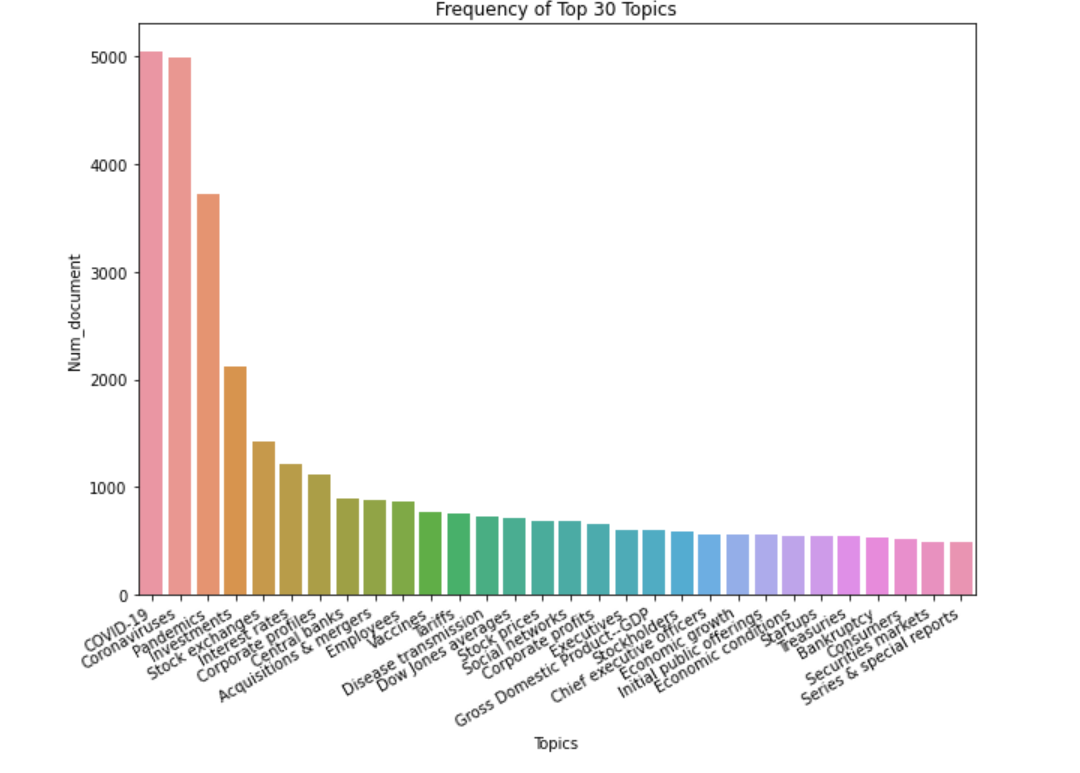
\includegraphics[width=15cm, height = 8cm]{graphs/topic_hist.PNG}
    \centering
    \caption{Frequency of Top 30 Topics}
    \label{Fig:topics}
    \end{figure}
    
    
    The monthly number of articles published fluctuates between $649$ and $1041$ with a notable increase after january of $2020$ when the pandemic was starting in the US. The inter-quartile range is $703$ to $797$. We can evidence the evolution of the number of articles in Figure \ref{Fig:number of articles}, the increase in both the number of tokens (words) and documents during the first months of $2020$ above their mean level (red dashed line) is evident. Furthermore, the average quantity of tokens in individual articles showed a steady increase over time with minor fluctuations, eventually rising significantly over the average level after february 2020. The sharp increase in the number of tokens after the second month of 2020 is similar to the trend of the number of articles during the same period, and could be caused by the onset of the covid-19 pandemic.
    
    
    \begin{figure}[H]
    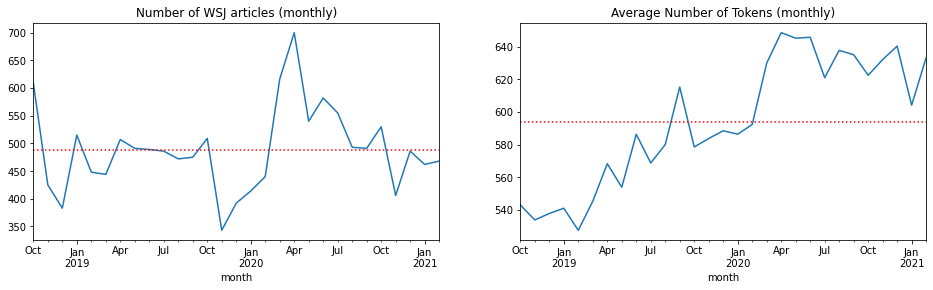
\includegraphics[width=15cm]{graphs/line_tokens.png}
    \centering
    \caption{Number of posts on Wall Street Journal(Monthly)}
    \label{Fig:number of articles}
    \end{figure}
    
    %\textcolor{red}{These plots could be added and discussed a) Scatter of realized Volatility against number of news per day (or maybe sum of the length of news from the day) b) Boxplot of number of news (maybe sum of the length of the news from the day) separated by direction}\\
    %\textcolor{red}{Can we do more interaction with the LDA results?
    %a) Barplot of topics that appear in Up or down days
    %b) Same as (a) but binning volatility in certain ranges and seeing if certain topics appear more c) Keyness plot}
    %\textcolor{red}{Remember that the modelling was done only using 2019-2020}
    
    The hypotheses that the number of tokens/types/sentences are the same for the articles that appear in days in which the market goes up and those in which it goes down cannot be rejected as the p-value of the t-statistics are $0.73$, $0.85$, $0.72$ respectively. When using log-likelihood for keyness analysis, the terms linked with downward-movement dates are losses, fallen, forced, and so on as shown in the word cloud below, whereas those related with upward-movement dates are sales, vaccine, and so on. Other obscure words, such as Wednesday and some entity names, occur in the UP day's word cloud and cannot be explained simply using the explanatory data analysis.
    
    \begin{figure}[H]
    \begin{subfigure}{.5\textwidth}
        \centering
        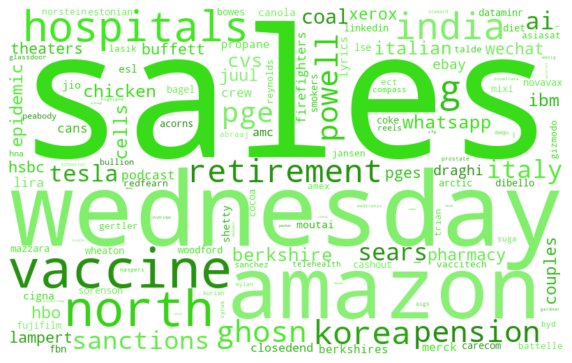
\includegraphics[width=1.0\linewidth]{graphs/upward_wordcloud1.png}
        \caption{Word Cloud of Up days}
    \end{subfigure}
    \begin{subfigure}{.5\textwidth}
        \centering
        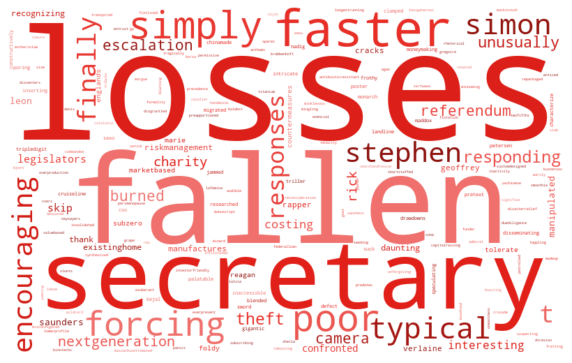
\includegraphics[width=1.0\linewidth]{graphs/downward_wordcloud1.png}
        \caption{Word Cloud of Down days}
    \end{subfigure}
    \end{figure}
    
    \begin{wrapfigure}{r}{0.5\textwidth}
        \begin{center}
            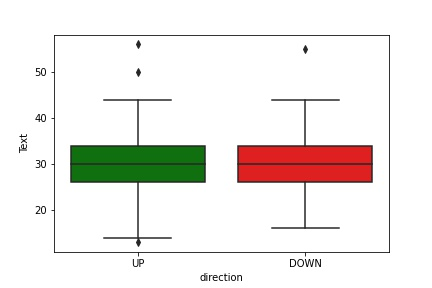
\includegraphics[width=0.48\textwidth]{graphs/dir_num1.jpg}
        \end{center}
        \caption{Number of Articles (daily)}
    \label{fig: dir}
    \end{wrapfigure}
    
    As for the correlation between the daily number of news and log variance of S{\&}P100, the linear correlation is not evident as shown in Figure \ref{fig: vol_num} if the outliers are not considered. On the other hand, the majority of the points in Figure \ref{fig: return_num} are laid around Return = 0, except for a few abnormal points. Also, the number of articles published on Up days and Down days are similar in terms of interquartile range, but the range of number of articles on Up days is slightly wider than that on Down days according to Figure \ref{fig: dir}.
    

    \begin{figure}[H]
    \begin{subfigure}{.5\textwidth}
        \centering
        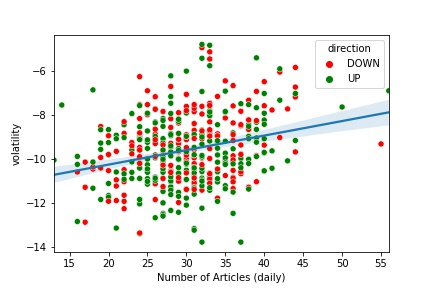
\includegraphics[width=1.0\linewidth]{graphs/vol_num1.jpg}
        \caption{Num of Articles VS Volatility}
        \label{fig: vol_num}
    \end{subfigure}
    \begin{subfigure}{.5\textwidth}
        \centering
        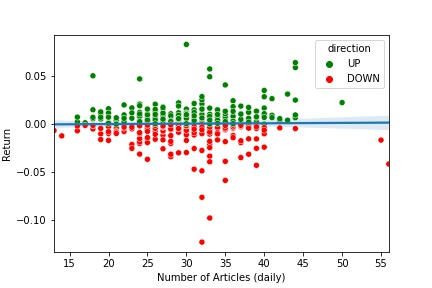
\includegraphics[width=1.0\linewidth]{graphs/return_num1.jpg}
        \caption{Num of Articles VS Return}
        \label{fig: return_num}
    \end{subfigure}
    \end{figure}
    
    %There is no obvious seasonal effect in the number of articles published every day except the fact that there were significantly more articles published daily in the second quarter of 2020, which aligns with the upward trend associated with COVID-19.(Figure \ref{Fig:boxplots wsj})
    
    %\begin{figure}[H]
    %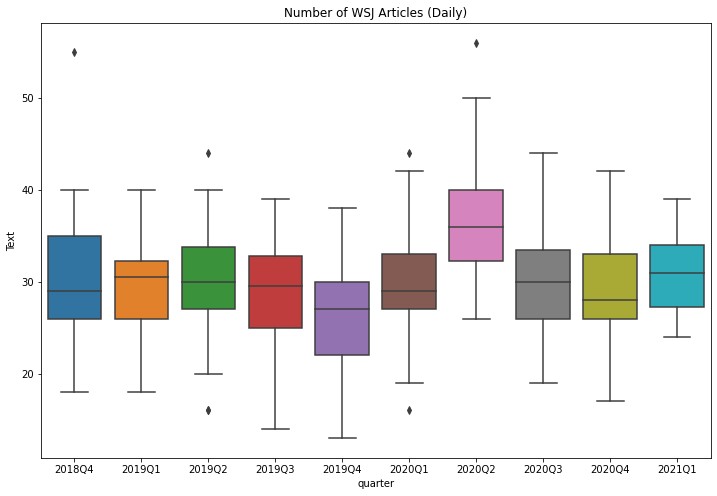
\includegraphics[width=15cm, height =  6cm]{graphs/seasonal.png}
    %\centering
    %\caption{Number of Articles Everyday}
    %\label{Fig:boxplots wsj}
    %\end{figure}
    \begin{wrapfigure}{r}{0.5\textwidth}
        \begin{center}
            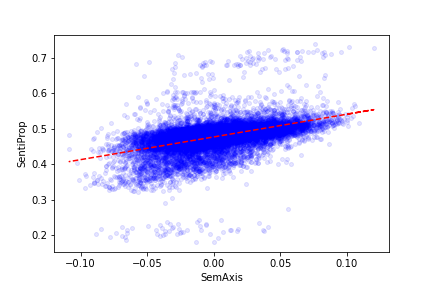
\includegraphics[width=0.48\textwidth]{graphs/words_ploar1.png}
        \end{center}
        \caption{Polarities of Words}
    \label{fig: words}
    \end{wrapfigure}
    
    Even though the polarities of each word derived by various approaches as shown in Table \ref{Tab: WSJ senti words} are in different scales, there is a positive correlation between average polarities derived by SemAxis and by SentiProp according to Figure \ref{fig: words}. The most positive words derived by SemAxis with various filtering conditions as well as different embeddings are ventures, investments, startup, etc. while that by SentiProp are risen, fund, investments, etc. According to this finding, the positive words tend to be related to investments and startups for both predictor generation methods. As for the most negative words,  they differ slightly when the embeddings and the methodologies are changed. The most negative words derived by both methods include but not are limited to medicine, worsen, eased, affect, etc.
    
    
    \section{Seeking Alpha}
    
    Seeking Alpha is a financial crowd-sourced content service that relies on contributions from a community of investors and industry experts rather than sell-side analysts. Its articles cover a broad range of stocks, asset classes, ETFs and investment strategies. 
    
    Seeking Alpha has stock markets news regarding different industries such as tech, energy and healthcare. We decided to work with a section named US markets since we believe it is the one that best covers the S$\&$P$100$ companies. For this project, $4716$ US market articles written between $1$ January $2019$ and $31$ December $2020$ were obtained using web scraping. We used Beautiful Soup and webdriver Python libraries to do this.  
    
    Before $2020$, the total number of articles per month was about $185$. When the number of covid-19 infections in the United States started to increase in March 2020, $426$ articles were released. A quarter later, the number of news returned to their normal values.
    
    \begin{figure}[H]
    \centering   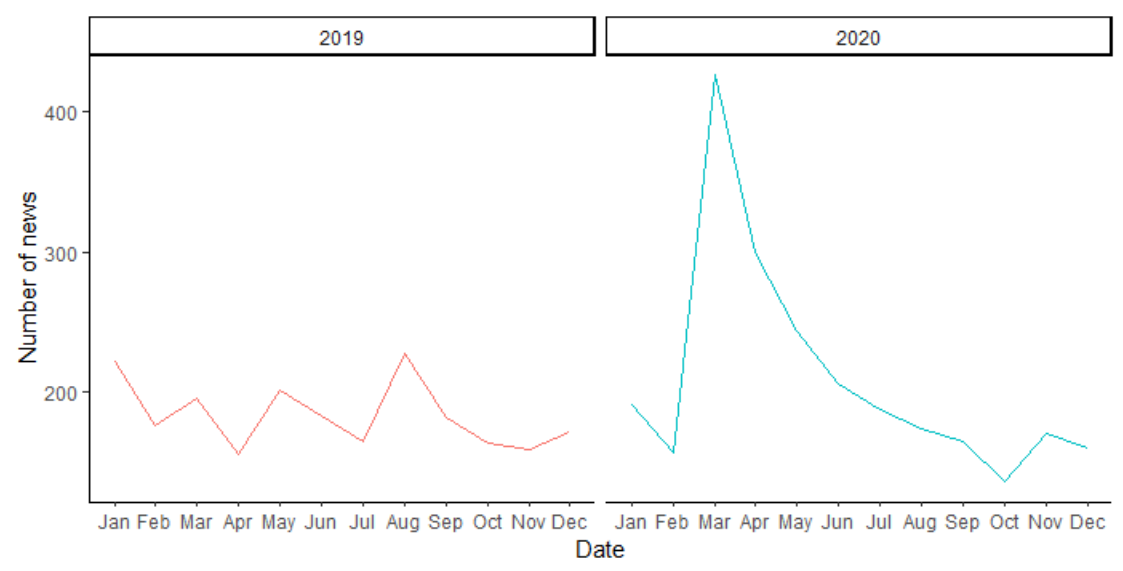
\includegraphics[width=14cm]{graphs/Seeking_Alpha/No_news_year.png}
    \caption{Number of news by month - Seeking Alpha}
    \label{Fig:No of news}
    \end{figure}
    
    If we join the news articles with the direction of the S$\&$P$100$ index the day the document was published, we can check the most frequent words when the market went up and down. To do this, we can use Keyness analysis, i.e., a relative frequency analysis to identify frequent words in news articles when the market went up, compared with the frequency of words when the market went down using the chi-squared test.
    
    
    The wordscloud in figure \ref{Fig:wordclouds_v2} shows that when the S$\&$P$100$ index went up, the most recurrent words are plus (+), up, new, gains, deal, and spending. There are words such as phase, (medical) treatment and reopening, which are positive due to the pandemic. On the other hand, the most repeated words when the index went down are US, down, coronavirus, government, negative, trading, and off. There are also some negative words due to the pandemic like flights (canceled) and coronavirus.
    
    \begin{figure}[H]
    \centering
    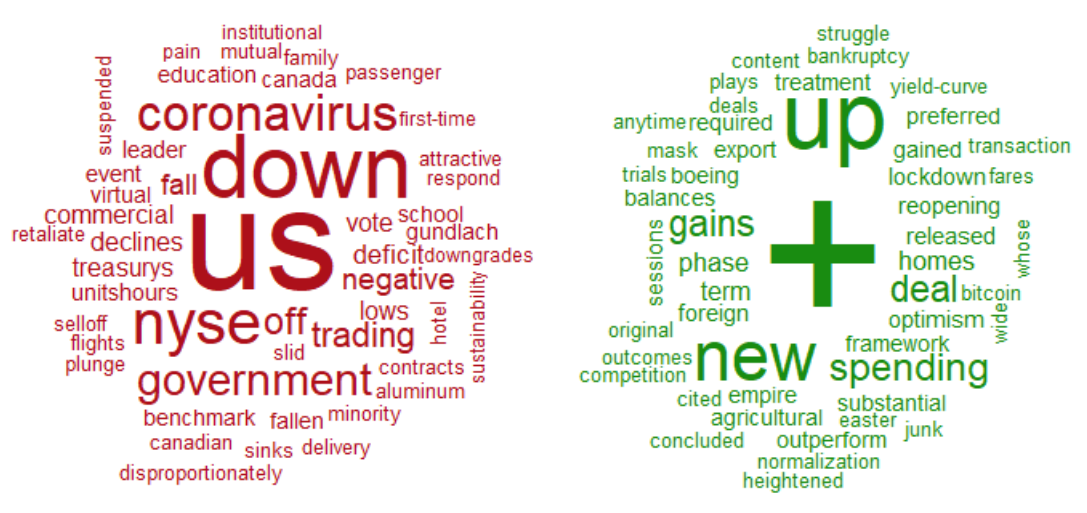
\includegraphics[width=14cm]{graphs/Seeking_Alpha/wordclouds_v2.png}
    \caption{Wordclouds of Up and Down days - Seeking Alpha}
    \label{Fig:wordclouds_v2}
    \end{figure}
    
    
    We can also summarize the documents and obtain the total number of words, punctuation marks, and numbers per news article. Each record has, on average, 138 words and 25 punctuation marks, i.e., 6 words per sentence. Seeking Alpha articles are short, like a paragraph long. In addition, each document includes 5 numbers, on average. Financial news need numbers to be more specific and accurate.
    
    In figure \ref{Fig:Boxplot_stats} we can observe boxplots of the number of words (tokens), punctuation marks and numbers by direction, Up and Down. It seems to be that there is no difference between the distributions of each direction. We can check this doing a test for differences between means. We can reject the hypothesis that the mean of the number of words and punctuation marks when the market went up is equal to the means when the market went down. The p-values are 0.0450 and 0.0385 respectively.  

    \begin{figure}[H]
    \centering
    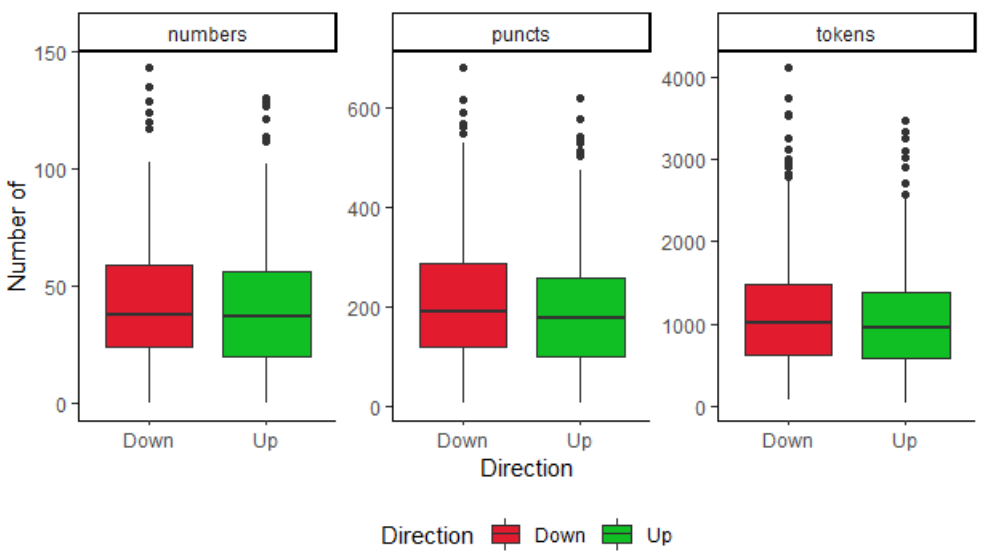
\includegraphics[scale=0.7]{graphs/Seeking_Alpha/Boxplot_stats.png}
    \caption{Boxplots of the number of words, punctuation marks and numbers by Direction}
    \label{Fig:Boxplot_stats}
    \end{figure}
    
    
    We can also explore the relation between the volatility and other features. In figure \ref{Fig:var_vs_tokens} we can see there is is weak positive relation between the volatility and the number of words of the news articles. While the number of tokens increase, the volatility will increase as well. However, there is no clear evidence of relation with the direction of the market.
    
    \begin{figure}[H]
    \centering
    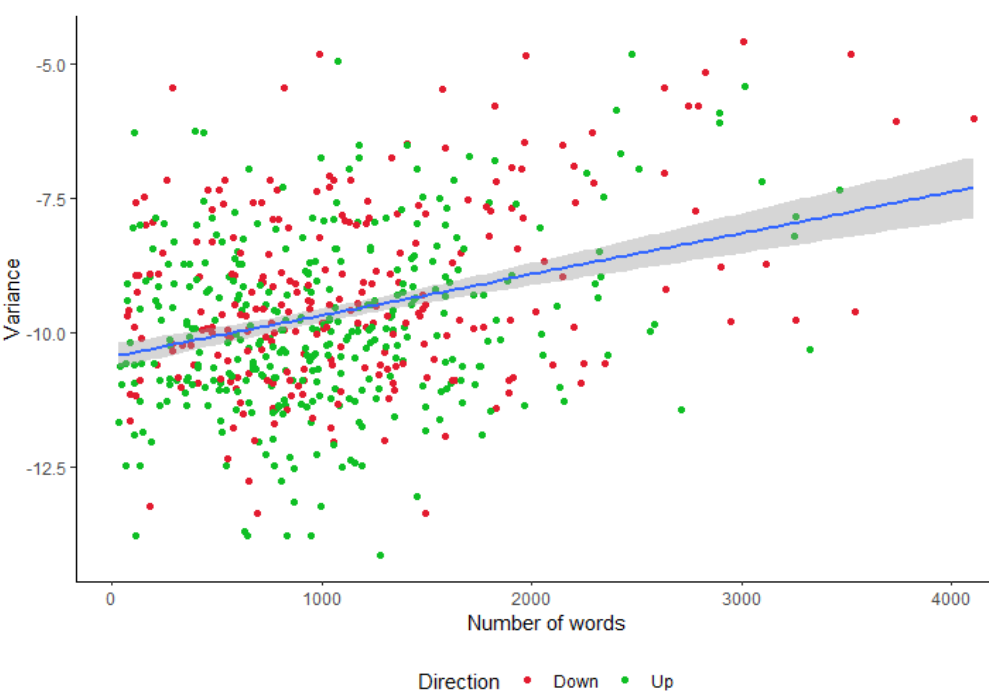
\includegraphics[scale=0.75]{graphs/Seeking_Alpha/var_vs_tokens.png}
    \caption{Number of words vs. Volatility - Seeking Alpha}
    \label{Fig:var_vs_tokens}
    \end{figure}
    
    
    If we divide the volatility by intervals, we can analyze the most frequent words by levels. The maximum volatility value is -$4.59$, and the minimum value is -$14.16$. The most recurrent positive words when the volatility is above -$8.5$ are almost all related to the pandemic such as covid, cases, hospitals, infectious, deaths, ventilators, masks, among others. The most repeated words when the volatility is between -$8.5$ and -$10.5$ are associated with economics and the contagion reduction like inflation, HPI, spending, revenue, recovery, vaccine, Moderna, efficacy, etc. Finally, the most common words when the volatility is below -$10.5$ are about production such as manufacturing, goods, trade, growth, construction, sales, consumer, and deal (see figure \ref{Fig:var_levels_sa}).
    
    \begin{figure}[H]
    \begin{subfigure}[t]{.32\textwidth}
        \centering
        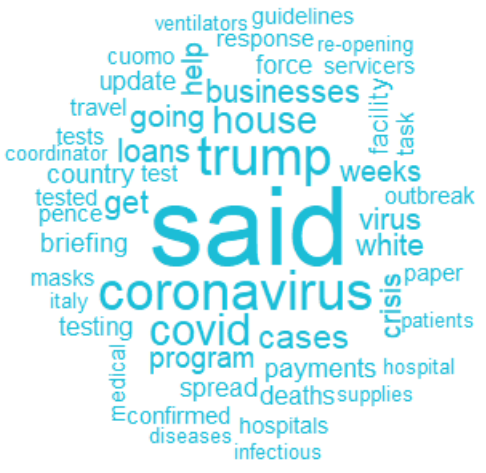
\includegraphics[width=\textwidth]{graphs/Seeking_Alpha/var_wordclouds_a.png}
        \caption{V > -8.5}
        \label{Fig:var_wordclouds_a}
    \end{subfigure}
    \begin{subfigure}[t]{.32\textwidth}
        \centering
        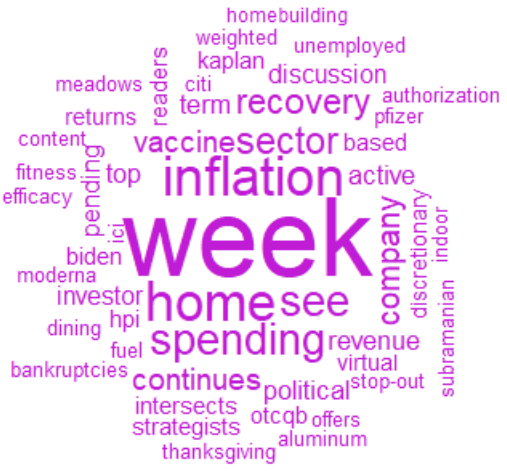
\includegraphics[width=\textwidth]{graphs/Seeking_Alpha/var_wordclouds_b.png}
        \caption{-10.5 < V < -8.5}
        \label{Fig:var_wordclouds_b}
    \end{subfigure}
    \begin{subfigure}[t]{.32\textwidth}
        \centering
        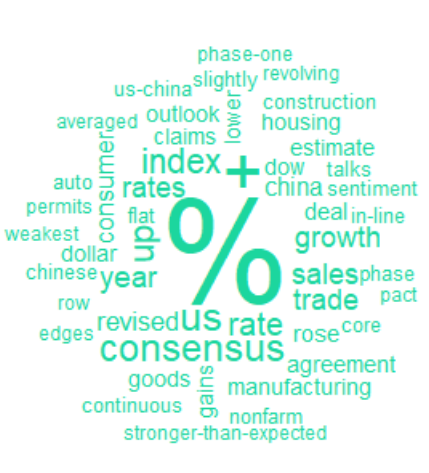
\includegraphics[width=\textwidth]{graphs/Seeking_Alpha/var_wordclouds_c.png}
        \caption{V < -10.5}
        \label{Fig:var_wordclouds_c}
    \end{subfigure}
    \caption{Realized volatility by levels - Seeking Alpha}
    \label{Fig:var_levels_sa}
    \end{figure}
    
    
    
    \section{Twitter}
    Twitter is a social network where users share their thoughts publicly in brief words. This posts, known as tweets, can be shared and commented by others, creating tendencies. We have $93959$ tweets obtained using web scraping.  The keywords used to filter the data were the hashtags {\#}index, {\#}usmarkets, {\#}s$\&$p100 and {\#}stockmarket between $1$ January $2019$ and $31$ December $2020$. The number of tweets have an increasing trend as shown in figure \ref{Fig:No_twits}. We can observe a peak in March 2020, when the pandemic began. 
    

    \begin{figure}[H]
    \centering
    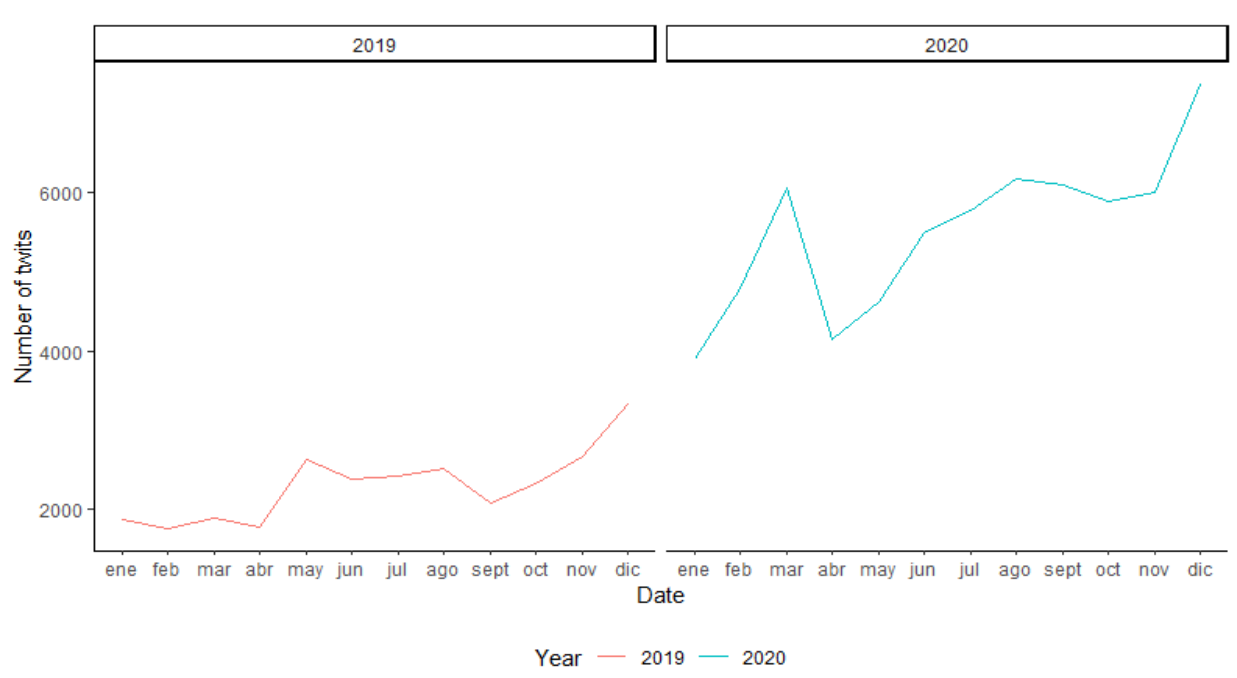
\includegraphics[scale=0.7]{graphs/Twitter/No_twits.png}
    \caption{Number of tweets}
    \label{Fig:No_twits}
    \end{figure}

    Figure \ref{Fig:pos_neg_wordclouds} illustrates the most relative frequent words when the market went up and down. The most recurrent words when the market went up are {\#}finance, + (plus), {\#}stocktips, {\#}sharetrading, {\#}smartmoney, gained, wealth and tariffs. On the other hand, the most repeated words when the market went down are {\#}coronavirus, {\#}covid, level, {\#}stockmarketcrash, news, lower, fall, sink, and drop. We can see also hashtags as {\#}blackmonday, discussed in the introduction of this document. 

    \begin{figure}[H]
    \centering
    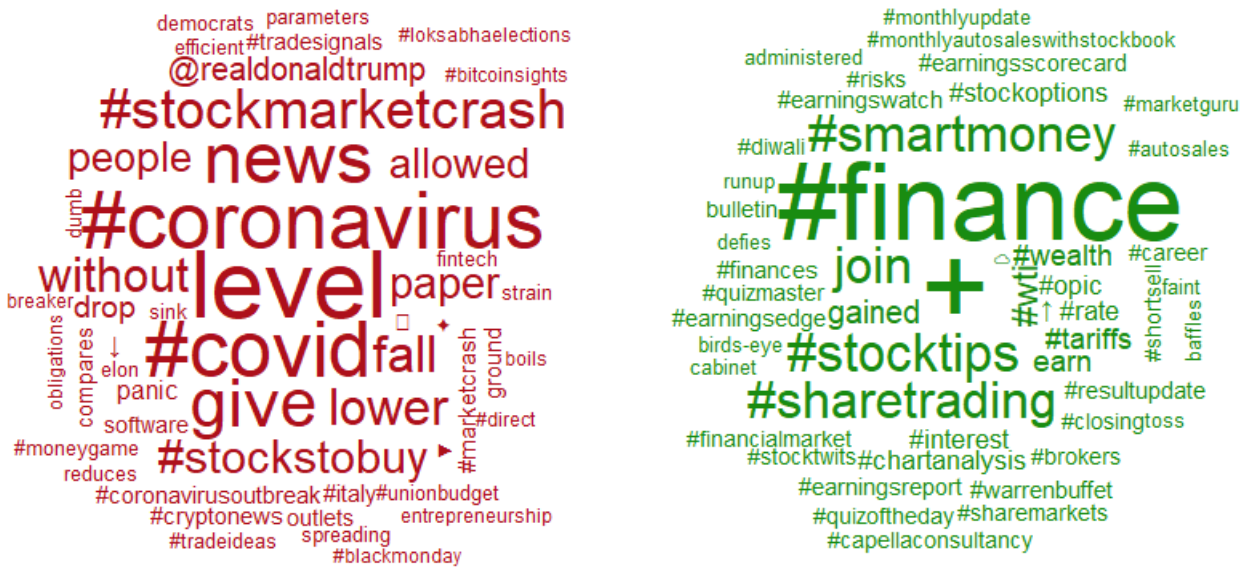
\includegraphics[scale=0.65]{graphs/Twitter/pos_neg_wordclouds.png}
    \caption{Wordclouds of Up and Down days - Twitter}
    \label{Fig:pos_neg_wordclouds}
    \end{figure}


    Tweets are limited on space. The maximum number of characters found is 779, i.e., around 120 words. In figure \ref{Fig:Boxplots_EDA} we can see boxplots of the number of characters, tokens (words), and types (unique words) by day, classified by direction, up and down. Using a test for differences between means,  we cannot reject the hypothesis that the mean of the number of characters, words and types when the market went up is equal to the mean when the market went down. The p-values are 0.2259, 0.1639 and 0.1859 respectively. 
    
    
    \begin{figure}[H]
    \centering
    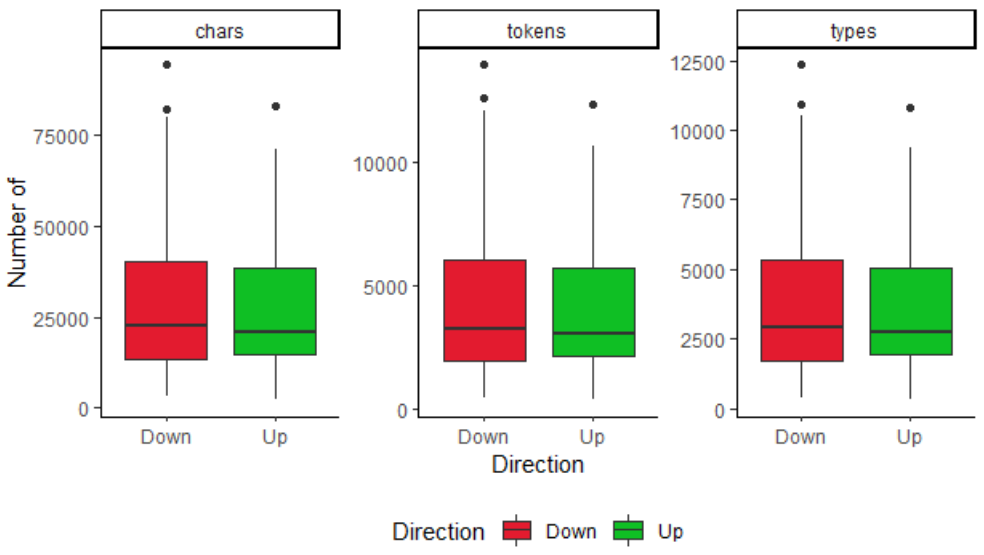
\includegraphics[scale=0.7]{graphs/Twitter/Boxplots_EDA.png}
    \caption{Boxplots of the number of characters, words and types by Direction}
    \label{Fig:Boxplots_EDA}
    \end{figure}
    
    Similarly to figure \ref{Fig:var_vs_tokens}, there is a weak positive correlation between the volatility and the number of words. However, there is no clear evidence of relationship with the direction of the market.

    \begin{figure}[H]
    \centering
    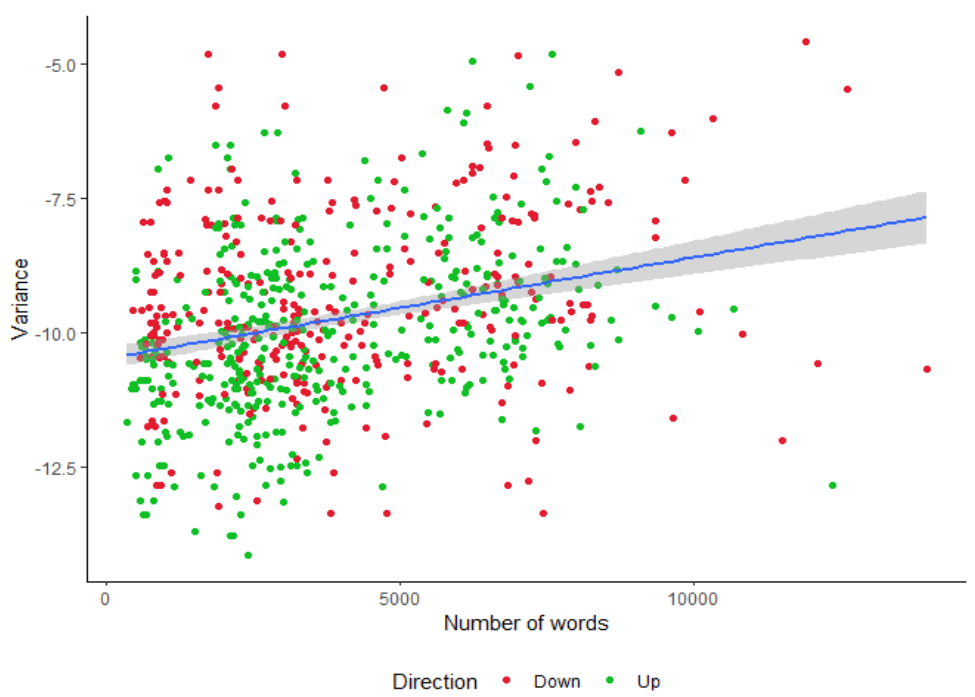
\includegraphics[scale=0.75]{graphs/Twitter/var_vs_tokens.png}
    \caption{Number of words vs. Volatility - Twitter}
    \label{Fig:Scatter_twt}
    \end{figure}
    
    
    Finally, we checked the most frequent words by levels of volatility. Homogeneously to figure \ref{Fig:var_wordclouds_a}, the most periodic terms when the volatility is above -8.5 are negative and linked to the pandemic. A few examples of them are covid, lockdown, recession, virus, crisis, panic, crash, plunge, fall, among others. For the medium and low levels shown in figure \ref{Fig:var_levels_tw}, the most constant words are connected to the stock market, such as investing, stop-loss, nasdaq, charts, finance, {\#}technicalanalysis, volatility, profits, volume, etc.
    
    \begin{figure}[H]
    \begin{subfigure}[t]{.32\textwidth}
        \centering
        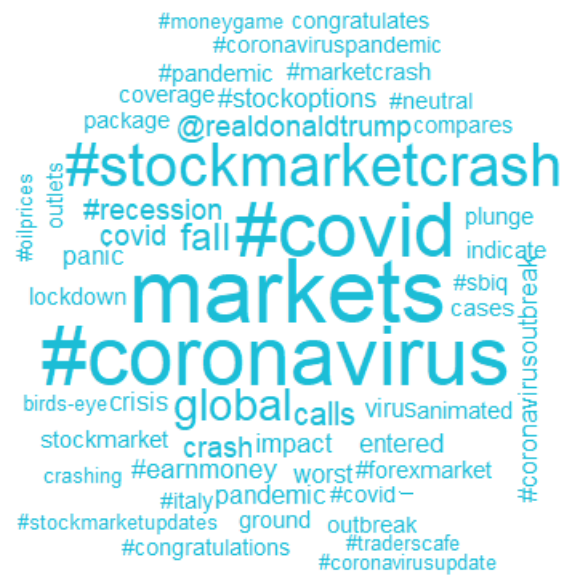
\includegraphics[width=\textwidth]{graphs/Twitter/var_wcloud_twt1.png}
        \caption{V > -8.5}
        \label{Fig:var_wcloud_twt1}
    \end{subfigure}
    \begin{subfigure}[t]{.32\textwidth}
        \centering
        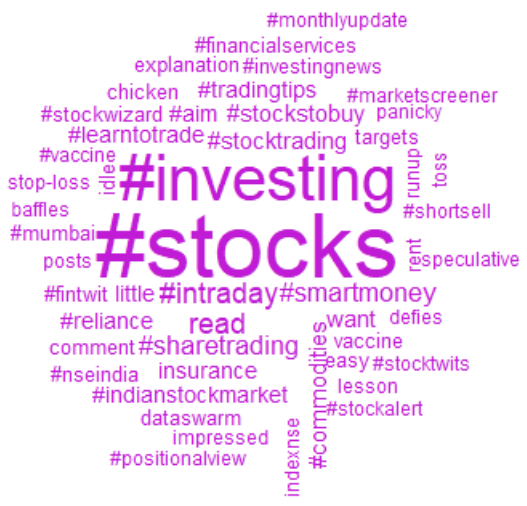
\includegraphics[width=\textwidth]{graphs/Twitter/var_wcloud_twt2.png}
        \caption{-10.5 < V < -8.5}
        \label{Fig:var_wcloud_twt2}
    \end{subfigure}
    \begin{subfigure}[t]{.32\textwidth}
        \centering
        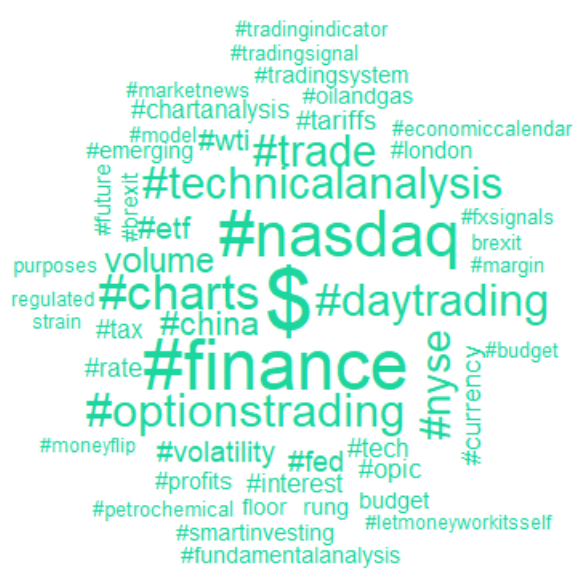
\includegraphics[width=\textwidth]{graphs/Twitter/var_wcloud_twt3.png}
        \caption{V < -10.5}
        \label{Fig:var_wcloud_twt3}
    \end{subfigure}
    \caption{Realized volatility by levels - Twitter}
    \label{Fig:var_levels_tw}
    \end{figure}
    
    \section{Financial Markets}
    
    In order to measure the effect of the news and tweets on the financial markets, we decided to use the S$\&$P$100$ as a broad measure of the financial markets. The decision was made considering that it includes the $100$ biggest companies traded in the United States. The top-10 companies by index weight include Apple, Microsoft, Amazon, Facebook, Google, Tesla, among others. Data of the index was obtained through the Yahoo Finance api.  
    
    We calculate the baseline returns using the difference in the logarithm of the original index. The direction is obtained by taking the sign of the returns for each day. The realized volatility is calculated by using 5-day sliding windows and computing the logarithm of the variance within each window. 
    
    
    Figure \ref{Fig:returns} illustrates the behaviour of the returns. The behaviour was relatively stable before march 2020, month in which several countries implemented a lockdown measure in order to curb the rising cases of covid-$19$. During this month, the index had daily increases of about $10$ percent and decreases of approximately $12$ percent with apparently erratic swings. We note that from april $2020$ onwards the index had a larger volatility than the one observed during $2019$.  This increase in volatility is probably linked to the uncertainty derived from the pandemic.
    
    
    \begin{figure}[H]
    \begin{subfigure}[t]{.64\textwidth}
        \centering
        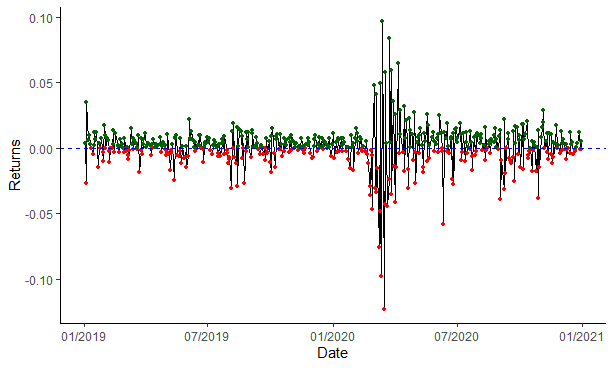
\includegraphics[width=\textwidth]{graphs/Returns.png}
        \caption{Daily Returns}
        \label{Fig:returns}
    \end{subfigure}
    \begin{subfigure}[t]{.34\textwidth}
        \centering
        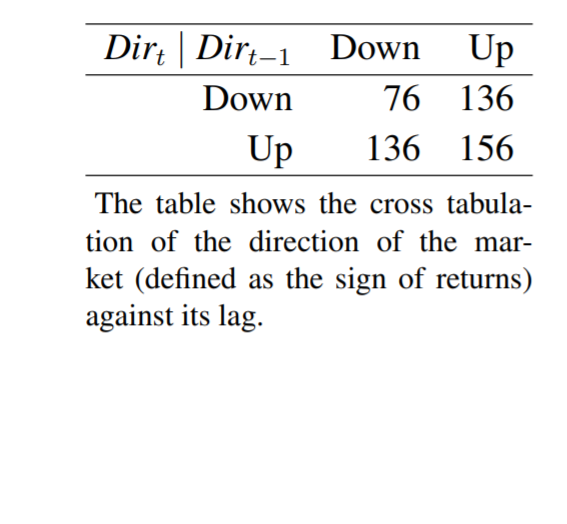
\includegraphics[width=\textwidth]{graphs/table_dir.png}
        \caption{Direction cross tabulation}
        \label{Fig:DirectionCross}
    \end{subfigure}
    \caption{S$\&$P100}
    \label{Fig:returns_crosstab}
    \end{figure}
    
    
    %%%% original code %%%
    %\begin{figure}[H]
    %\centering
    %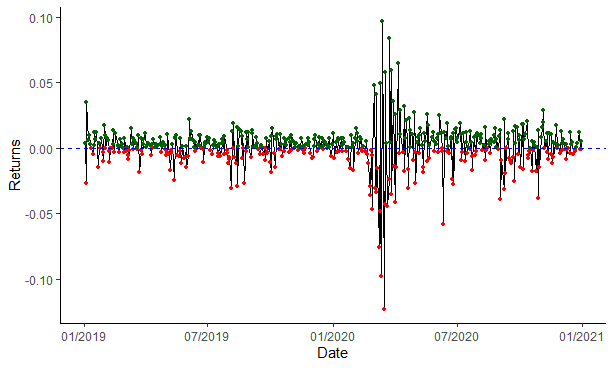
\includegraphics[scale = 0.6]{graphs/Returns.png}
    %\caption{Daily Returns - S$\&$P100}
    %\label{Fig:returns}
    %\end{figure}
    
    %\begin{table}[H]
    %\setlength{\columnwidth}{1pt}
    %\centering
    %\begin{threeparttable}
   %\begin{tabular}{rrr}
    %  \hline
     %\textit{Dir$_t$} $|$ \textit{Dir$_{t-1}$} & Down & Up \\ 
     % \hline
    %Down &  76 & 136 \\
    % Up & 136 & 156 \\ 
    %   \hline
    %\end{tabular}
    %\begin{tablenotes}
     % \footnotesize
      %\item The table shows the cross tabulation of the direction of the market (defined as the sign of returns) against its lag.
    %\end{tablenotes}
    %\caption{Direction cross tabulation}
    %\label{Tab:DirectionCross}
  %\end{threeparttable}
   % \end{table}
    
    Table \ref{Fig:DirectionCross} shows the cross tabulation obtained by crossing the Direction and its lag. The null hypothesis of independence is rejected using a chi-squared independence statistic. Suggesting evidence of first order autocorrelation in the direction series. 
    
    Figure \ref{Fig:returnsseason} shows a daily seasonal bar plot of the proportions of both up and down days in the returns of the S$\&$P$100$. Though there are evident differences in the proportions. they aren't statistically significant as all the error bars overlap. 
    
    \begin{figure}[H]
    \centering
    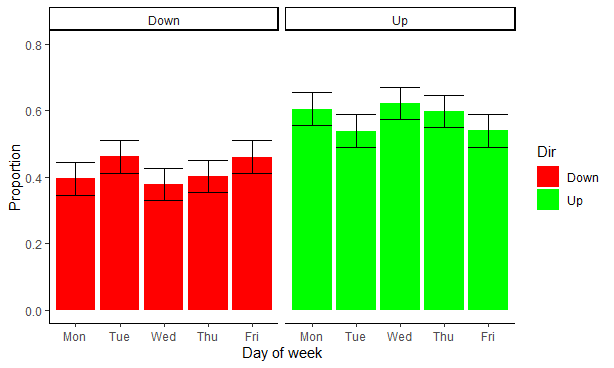
\includegraphics[scale = 0.65]{graphs/DirSeasonalEffects.png}
    \caption{S$\&$P100 daily seasonal effects on direction}
    \label{Fig:returnsseason}
    \end{figure}
    
    Figure \ref{Fig:variance} below shows the realized volatility series calculated using 5-day sliding variance windows. The red line is interpreted as the underlying trend and is calculated using a long-span Henderson filter. As can be seen in the plot, there is an evident increase in the volatility during the start of the second quarter of $2020$. Period in which most economies had to put a halt in production and declare country wide lockdowns to curb the rise of covid-19 infections. The highest points are reached in the second week of march just before the generalized lockdown measures were brought forward.  There is an evident decrease in the series in the summer of $2020$ when most developed economies reopened as they overcame the first wave of covid-19 cases. 
    
        \begin{figure}[H]
    \begin{subfigure}[t]{.5\textwidth}
        \centering
        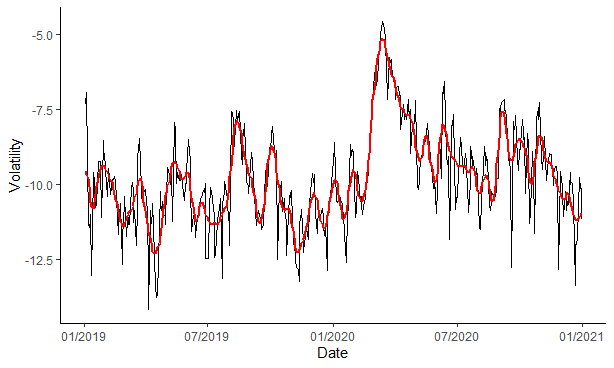
\includegraphics[width=\textwidth]{graphs/Variance.png}
        \caption{Volatility}
        \label{Fig:variance}
    \end{subfigure}
    \begin{subfigure}[t]{.5\textwidth}
        \centering
        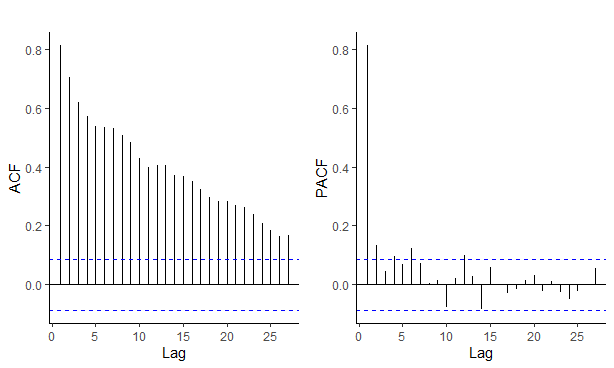
\includegraphics[width=\textwidth]{graphs/Variance_ACF.png}
        \caption{Volatility ACF and PACF}
        \label{Fig:varianceacf}
    \end{subfigure}
    \caption{S$\&$P100}
    \label{Fig:variance_plots}
    \end{figure}
    
    %%% Original Code %%
    %\begin{figure}[H]
    %\centering
    %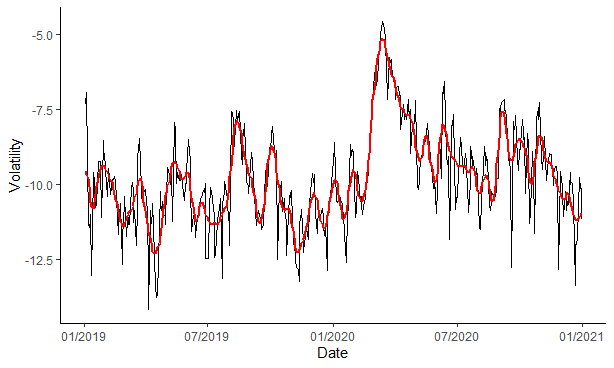
\includegraphics[scale = 0.6]{graphs/Variance.png}
    %\caption{S$\&$P100 volatility}
    %\label{Fig:variance}
    %\end{figure}
    
        
    %\begin{figure}[H]
    %\centering
    %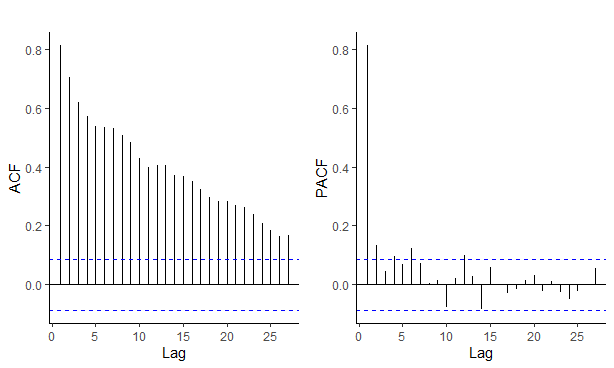
\includegraphics[scale = 0.6]{graphs/Variance_ACF.png}
    %\caption{S$\&$P100 volatility ACF and PACF}
    %\label{Fig:varianceacf}
    %\end{figure}
    
    Figure \ref{Fig:varianceacf} shows both the ACF and PACF of the realized volatility series. As both plots suggest, there is autocorrelation in the series. The tapering off in the ACF and the one/two significant bars in the PACF suggest that the autocorrelation in the series can be modelled as an AR(1) or AR(2) process. In both cases the resulting residual series are white noise, though the AR(2) model is preferred by the AIC. 

    
    %There is no apparent presence of daily seasonal effects in the realized volatility series as can be seen in figure \ref{Fig:varianceseasonal}. The distribution of the volatility across different days is almost identical. 
    
    %\begin{figure}[H]
    %\centering
    %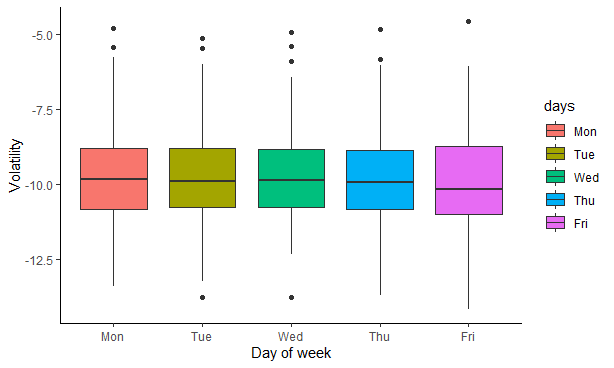
\includegraphics[scale = 0.5]{graphs/VolSeasonalEffects.png}
    %\caption{S$\&$P100 daily seasonal effects on volatility}
    %\label{Fig:varianceseasonal}
    %\end{figure}
   
    
 
    
    \newpage
    \chapter{Results}
    \section{Direction}
    \label{Sec:Dir}
    In this section we discuss the results of all the combinations of models mentioned in the modelling section (\ref{model}), and the different methods to derive the set of predictors. The methods considered are a Baseline model with no text predictors (No Regs), sentiment analysis series derived from the dictionary proposed in \textcite{Loughran:2011} (McDonald), an analogous series but based on an inducted dictionary using both the Semantic Axis and the SentiProp methodologies, a method based directly on Doc2Vec word embeddings, and another one that mirrors the application in \textcite{Gupta:2020}. All these methods are discussed in section \ref{predictor}. Models considered include AdaBoost (ADA), GLM $+$ AIC, Random Forest (RF) and a Support Vector Machine (SVM). For each of the methods mentioned above we consider each of these models. 
    
    The problem of predicting the direction of the market is framed as a classification problem. The results of the evaluation with a random held-out set are presented in table \ref{Tab:acc cv}. In terms of accuracy, the baseline SVM model without regressors, the SVM using the Doc2Vec predictors and the SVM based on the sentiment series derived from the SentiProp algorithm achieve the best results. It is important to note that the direction is slightly unbalanced in the complete sample as $58\%$ of the observations correspond to the up label. The imbalance is even more notorious in the basic hold-out set as $66\%$ of the observations correspond to the up label. The corresponding number for the last 3-month holdout is $51\%$. 
    
    The imbalance can be seen by looking at the precision metric, as the most accurate models are not the ones that have the highest precision, but they do have a perfect recall. This Suggests that they predict positive more often that the rest of models considered.  
    
    
    The F1 Score, which conveys the balance between the precision and the recall, shows that three combinations of models and methods are the top performers, achieving a score of $0.80$. The methods are the SentiProp, Doc2Vec and baseline without text information, all using the SVM model. This suggests that, at least for the sample considered, the decision boundary for the classification task is moderately nonlinear and weakly dependent on the text features. The nonlinearity follows as the SVM model we considered is based on radial basis kernels. 
    
    %As we are going to construct a profitable portfolio with the prediction, accuracy is the most important matrix in this case. The bar charts \ref{Fig:Accuracy}, \ref{Fig:F1} illustrate the Accuracy and F1 Score of the best combination of methods and models.
    
    \begin{table}[H]
    \setlength{\columnwidth}{1pt}
    \centering
    \begin{threeparttable}
   \begin{tabular}{rrrrrrrrrrr}
      \hline
     & & \textbf{Acc} & \textbf{Pr} & \textbf{Rec} & \textbf{F1} & & \textbf{Acc} & \textbf{Pr} & \textbf{Rec} & \textbf{F1} \\ 
      \midrule
      \multirow{8}{*}{\textbf{Baseline}} & & \multicolumn{4}{c}{\textbf{No Regs}} & & \multicolumn{4}{c}{\textbf{McDonald}} \\
      \cmidrule{3-11}\\
      & \textit{ADA} & 0.52 & 0.63 & 0.67 & 0.65 & & 0.55 & 0.65 & 0.70 & 0.68  \\ 
      & \textit{GLM} + \textit{AIC} &  0.55 & 0.63 & 0.81 & 0.71 & & 0.54 & 0.64 & 0.72 & 0.68  \\ 
      & \textit{RF} & 0.54 & 0.64 & 0.70 & 0.67 & & 0.55 & 0.66 & 0.67 & 0.67\\ 
      & \textit{SVM} & \textbf{0.66} & 0.66 & \textbf{1.00} & \textbf{0.80} & & 0.53 & 0.64 & 0.70 & 0.67 \\ 
      \multicolumn{9}{c}{} \\
      \multirow{8}{*}{\textbf{ID}} & & \multicolumn{4}{c}{\textbf{SemAxis}} & & \multicolumn{4}{c}{\textbf{SentiProp}} \\
      \cmidrule{3-11}\\
       & \textit{ADA} & 0.56 & 0.66 & 0.70 & 0.68 & & 0.64 & 0.69 & 0.84 & 0.76\\ 
      & \textit{GLM} + \textit{AIC} & 0.53 & 0.64 & 0.67 & 0.66 & & 0.59 & 0.67 & 0.78 & 0.72 \\ 
      & \textit{RF} &  0.52 & 0.63 & 0.69 & 0.66 & & 0.63 & \textbf{0.71} & 0.76 & 0.73 \\ 
      & \textit{SVM} & 0.62 & 0.69 & 0.79 & 0.74 & & \textbf{0.66} & 0.66 & \textbf{1.00} & \textbf{0.80} \\
      \multicolumn{9}{c}{} \\
      \multirow{8}{*}{\textbf{Doc2Vec}} & & \multicolumn{4}{c}{\textbf{Doc2Vec}} & & \multicolumn{4}{c}{\textbf{Gupta}} \\
       \cmidrule{3-11}\\
      & \textit{ADA} & 0.54 & 0.64 & 0.72 & 0.68 & \multicolumn{5}{c}{} \\ 
      & \textit{GLM} + \textit{AIC} & 0.53 & 0.65 & 0.66 & 0.65 & \multicolumn{5}{c}{} \\ 
      & \textit{RF} & \textbf{0.66} & 0.67 & 0.97 & 0.79 &  \multicolumn{5}{c}{}\\ 
      & \textit{SVM} & \textbf{0.66} & 0.66 & \textbf{1.00} & \textbf{0.80}& & 0.55 & 0.65 & 0.67 & 0.66\\
       \bottomrule
    \end{tabular}
    \begin{tablenotes}
      \footnotesize
      \item GLM + AIC method is based on a stepwise selection procedure applied to a GLM model. ADA is used to denote the Ada Boost model. RF stands for the random forest model and SVM for support vector model. The \textcite{Gupta:2020} is strictly SVM based so no other combination can be implemented. ID stands for inducted dictionary methods. The four statistical metrics measured are accuracy, precision, recall and F1.
    \end{tablenotes}
    \caption{Direction prediction regular holdout}
    \label{Tab:acc cv}
  \end{threeparttable}
    \end{table}
    
    %   \begin{figure}[H]
    % \begin{subfigure}{.5\textwidth}
    %     \centering
    %     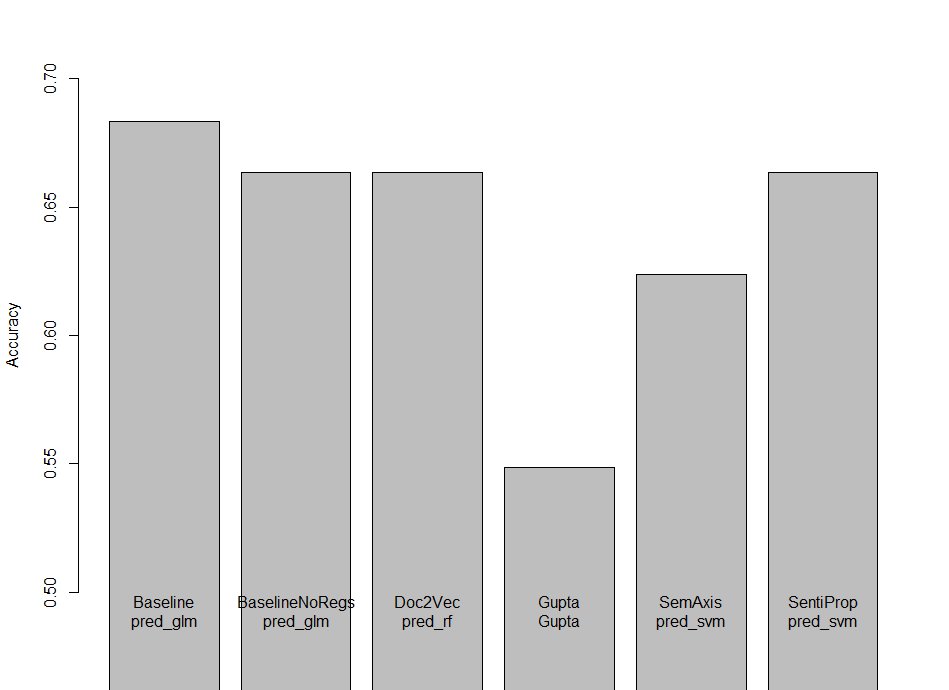
\includegraphics[width=.8\linewidth]{graphs/accuracy.png}
    %     \caption{Classification Accuracy}
    %     \label{Fig:Accuracy}
    % \end{subfigure}
    % \begin{subfigure}{.5\textwidth}
    %     \centering
    %     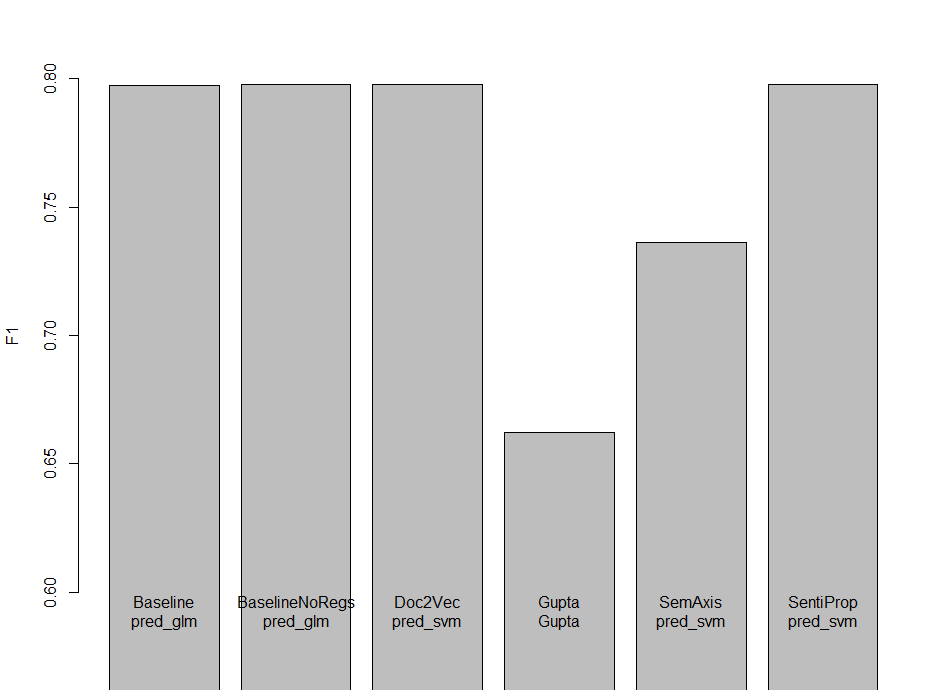
\includegraphics[width=.8\linewidth]{graphs/f1.png}
    %     \caption{The F1 Score of Classification models}
    %     \label{Fig:F1}
    % \end{subfigure}
    % \end{figure}
    
    Figure \ref{Fig:diragg} presents the metrics obtained in Table \ref{Tab:acc cv} aggregated both by model and by method. The aggregation is done using an average over each metric, except for the $F1$ metric which is recalculated based on the precision and recall values obtained. For example, the number $0.6$ presented for the accuracy metric of the Doc2Vec method is obtained by averaging all the results for the different models (namely, ADA, GLM $+$ AIC, RF and SVM) in the Doc2Vec method piece of table \ref{Tab:acc cv}. Similarly, the accuracy score presented for the SVM model is obtained by averaging the results for this model across all methods (No Regs, McDonald, SemAxis, etc.). We observe that the SentiProp method achieves better metrics across all the models considered and hence is the best method in this regard. In terms of models, the SVM achieves higher metrics than the others considered. In particular, the additional gain in recall by using this model is close to $10\%$ above the levels of the other models. 
    
    \begin{figure}[H]
    \centering
    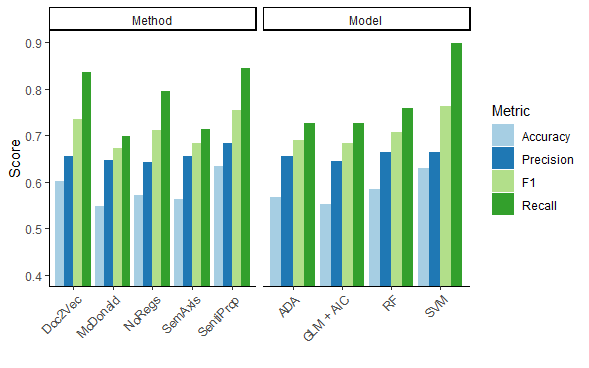
\includegraphics[scale = 0.7]{graphs/Dir_Agg.png}
    \caption{Direction aggregated metrics}
    \label{Fig:diragg}
    \end{figure}
    
    
    The models are also evaluated on a different hold out set that only includes the last three months in the sample to showcase their applicability (see table \ref{Tab:acc cv3}) . In this case, the GLM + AIC model with the sentiment series generated by SemAxis as predictor achieved the highest accuracy (60$\%$). Overall, the accuracy with this new holdout set is below the one achieved with the random holdout set evaluated before, but the reason behind might be the initial label imbalance. Considering the F1 Score, five combinations of models and methods attained the highest score of $0.69$. These were the SVM with SemAxis, GLM+AIC with SentiProp, Random Forest with SentiProp, Random Forest with Doc2Vec, and SVM with Doc2Vec. 
    
    % Both of the results are lower than that in the previous cross validation approach, which indicate the limitation of the these models' applicability.
    
     \begin{table}[H]
    \setlength{\columnwidth}{1pt}
    \centering
    \begin{threeparttable}
   \begin{tabular}{rrrrrrrrrrr}
      \hline
     & & \textbf{Acc} & \textbf{Pr} & \textbf{Rec} & \textbf{F1} & & \textbf{Acc} & \textbf{Pr} & \textbf{Rec} & \textbf{F1} \\ 
      \midrule
      \multirow{8}{*}{\textbf{Baseline}} & & \multicolumn{4}{c}{\textbf{No Regs}} & & \multicolumn{4}{c}{\textbf{McDonald}} \\
      \cmidrule{3-11}\\
      & \textit{ADA} & 0.48 & 0.50 & 0.75 & 0.60 & & 0.49 & 0.51 & 0.93 & 0.66   \\ 
      & \textit{GLM} + \textit{AIC} &  0.52 & 0.52 & \textbf{1.00} & 0.68 & & 0.53 & 0.53 & 0.89 & 0.66   \\ 
      & \textit{RF} & 0.54 & 0.54 & 0.86 & 0.66 & & 0.54 & 0.53 & 0.89 & 0.67\\ 
      & \textit{SVM} & 0.52 & 0.52 & \textbf{1.00} & 0.68 & & 0.52 & 0.52 & 1.00 & 0.68  \\ 
      \multicolumn{9}{c}{} \\
      \multirow{8}{*}{\textbf{ID}} & & \multicolumn{4}{c}{\textbf{SemAxis}} & & \multicolumn{4}{c}{\textbf{SentiProp}} \\
      \cmidrule{3-11}\\
       & \textit{ADA} & 0.48 & 0.50 & 0.86 & 0.63 & & 0.52 & 0.52 & 0.89 & 0.66 \\ 
      & \textit{GLM} + \textit{AIC} & 0.55 & 0.54 & 0.89 & 0.67 & & \textbf{0.60} & \textbf{0.58} & 0.84 & \textbf{0.69}  \\ 
      & \textit{RF} & 0.49 & 0.51 & 0.91 & 0.65 & & 0.53 & 0.52 & \textbf{1.00} & \textbf{0.69} \\ 
      & \textit{SVM} & 0.56 & 0.55 & 0.93 & \textbf{0.69} & & 0.52 & 0.52 & \textbf{1.00} & 0.68  \\
      \multicolumn{9}{c}{} \\
      \multirow{8}{*}{\textbf{Doc2Vec}} & & \multicolumn{4}{c}{\textbf{Doc2Vec}} & & \multicolumn{4}{c}{\textbf{Gupta}} \\
       \cmidrule{3-11}\\
      & \textit{ADA} & 0.53 & 0.53 & 0.91 & 0.67  & \multicolumn{5}{c}{} \\ 
      & \textit{GLM} + \textit{AIC} & 0.53 & 0.53 & 0.70 & 0.61 & \multicolumn{5}{c}{} \\ 
      & \textit{RF} & 0.53 & 0.52 & \textbf{1.00} & \textbf{0.69} &  \multicolumn{5}{c}{}\\ 
      & \textit{SVM} & 0.54 & 0.53 & \textbf{1.00} & \textbf{0.69} & & 0.49 & 0.5 & 0.79 & 0.61\\
       \bottomrule
    \end{tabular}
    \begin{tablenotes}
      \footnotesize
      \item GLM + AIC method is based on a stepwise selection procedure applied to a GLM model. ADA is used to denote the Ada Boost model. RF stands for the random forest model and SVM for support vector model. The \textcite{Gupta:2020} is strictly SVM based so no other combination can be implemented. ID stands for inducted dictionary methods. The four statistical metrics measured are accuracy, precision, recall and F1.
    \end{tablenotes}
    \caption{Direction prediction last three months holdout}
    \label{Tab:acc cv3}
  \end{threeparttable}
    \end{table}
    
    The above average results obtained by changing the holdout sample are a reflection of the difference in the imbalance of the test sets. Using the regular hold-out set, we note that the best accuracy obtained is the same as the no-information rate while for the last three months hold out the accuracy is almost $9\%$ points higher. We do note a slight reduction in the precision of the classifiers when changing the hold out sample. 
    
    
    \section{Volatility}
    
    For the prediction of the volatility, we use the same models and methods as the ones discussed in the section above. The only exception is that the Ada Boost model is replaced by a multivariate adaptive regression spline with generalized cross validation selection (MARS). Results for the regular hold out set are presented in table \ref{Tab:Volatility2}. Among all the models, the best results are obtained using the GLM + AIC model with the predictors derived from SemAxis and the SVM model with predictors based on the sentiment series derived from the \textcite{Loughran:2011} dictionary. Both combinations achieved the highest $R^2$ (0.71) and the lowest RMSE (0.85). The Doc2Vec method is by far the worst performing one, as the $R^2$ is almost $0.2$ points below the ones obtained with the other methods, and the RMSE is almost one fourth bigger. %Figures \ref{Fig:RMSE} and \ref{Fig:RSquared} show a comparison of the metrics. 
    
    %the following bar charts \ref{Fig:RMSE}, \ref{Fig:RSquared}. This means that this method explains the largest proportion of the variance of the sentiment score derived from SexAxis, and gives the predicted volatility that is closest to the true volatility.
    
    \begin{table}[H]
    \centering
    \begin{threeparttable}
   \begin{tabular}{rrrrrrrrr}
      \hline
     & & \textbf{RMSE} & \textbf{R}$^2$ & \textbf{MAE} & & \textbf{RMSE} & \textbf{R}$^2$ & \textbf{MAE}\\ 
      \midrule
      \multirow{8}{*}{\textbf{Baseline}} & & \multicolumn{3}{c}{\textbf{No Regs}} & & \multicolumn{3}{c}{\textbf{McDonald}} \\
      \cmidrule{3-9}\\
      & \textit{GLM} + \textit{AIC} & 0.87 & 0.70 & 0.61 & & 0.89 & 0.69 & 0.62 \\ 
      & \textit{MARS} &  0.90 & 0.67 & 0.62 & & 0.96 & 0.64 & 0.67 \\ 
      & \textit{RF} & 0.86 & \textbf{0.71} & 0.63 & & 0.92 & 0.66 & 0.66 \\ 
      & \textit{SVM} & 0.87 & 0.70 & \textbf{0.59} & & \textbf{0.85} & \textbf{0.71} & 0.62 \\ 
      \multicolumn{9}{c}{} \\
      \multirow{8}{*}{\textbf{ID}} & & \multicolumn{3}{c}{\textbf{SemAxis}} & & \multicolumn{3}{c}{\textbf{SentiProp}} \\
      \cmidrule{3-9}\\
       & \textit{GLM} + \textit{AIC} & \textbf{0.85} & \textbf{0.71} & 0.60 & & 0.86 & 0.70 & 0.62 \\ 
      & \textit{MARS} & 0.92 & 0.67 & 0.67 & & 0.88 & 0.69 & 0.64 \\ 
      & \textit{RF} &  0.87 & 0.69 & 0.62 & & 0.89 & 0.68 & 0.64 \\ 
      & \textit{SVM} & 0.86 & \textbf{0.71} & 0.62 & & 0.87 & 0.70 & 0.61 \\
      \multicolumn{9}{c}{} \\
      \multirow{8}{*}{\textbf{Doc2Vec}} & & \multicolumn{3}{c}{\textbf{Doc2Vec}} & & \multicolumn{3}{c}{\textbf{}} \\
       \cmidrule{3-9}\\
      & \textit{GLM} + \textit{AIC} & 1.26 & 0.41 & 0.98 & \multicolumn{4}{c}{} \\ 
      & \textit{MARS} & 1.44 & 0.32 & 1.02 & \multicolumn{4}{c}{} \\ 
      & \textit{RF} & 1.09 & 0.53 & 0.83 &  \multicolumn{4}{c}{}\\ 
      & \textit{SVM} & 1.20 & 0.42 & 0.97 & \multicolumn{4}{c}{}\\
       \bottomrule
    \end{tabular}
    \begin{tablenotes}
      \footnotesize
      \item GLM + AIC method is based on a stepwise selection procedure applied to a GLM model. MARS is used to denote the multivariate adaptive regression splines algorithm with generalized cross-validation selection. RF stands for the random forest model and SVM for support vector model. ID stands for induced dictionary methods.
    \end{tablenotes}
    \caption{Volatility prediction regular holdout}
    \label{Tab:Volatility}
  \end{threeparttable}
    \end{table}
    
    We present the results aggregated by both method and model in Figure \ref{Fig:volagg}. The figure evidences the underperformance obtained by using the Doc2Vec method. While this method is the most flexible, we believe the high-dimensionality of its document representations (50-dimensional) and the low sample size over which the model is trained, (close to $600$ observations) explains why the results are worst than with other methods that carry out a more strict dimensionality reduction. The rest of methods considered achieve very similar results in terms of both RMSE and MAE. In terms of model choices, the figure evidences that most achieve similar results except for the MARS. We believe that the underperformance of this method again follows from the excess of flexibility and the small sample size over which the model is trained. Note also that the small sample is not an easy to solve problem as the covid-19 pandemic generated evident breaks in the series and it's reasonable to assume that coefficient instability during this period might be present. 
    
    \begin{figure}[H]
    \centering
    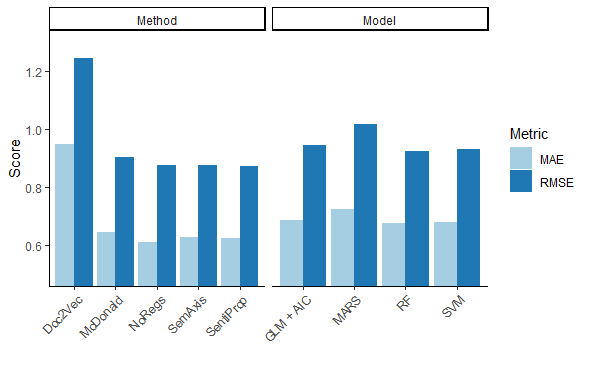
\includegraphics[scale = 0.7]{graphs/Vol_Agg.png}
    \caption{Volatility aggregated metrics}
    \label{Fig:volagg}
    \end{figure}
        
    % \begin{figure}[H]
    % \begin{subfigure}{.5\textwidth}
    %     \centering
    %     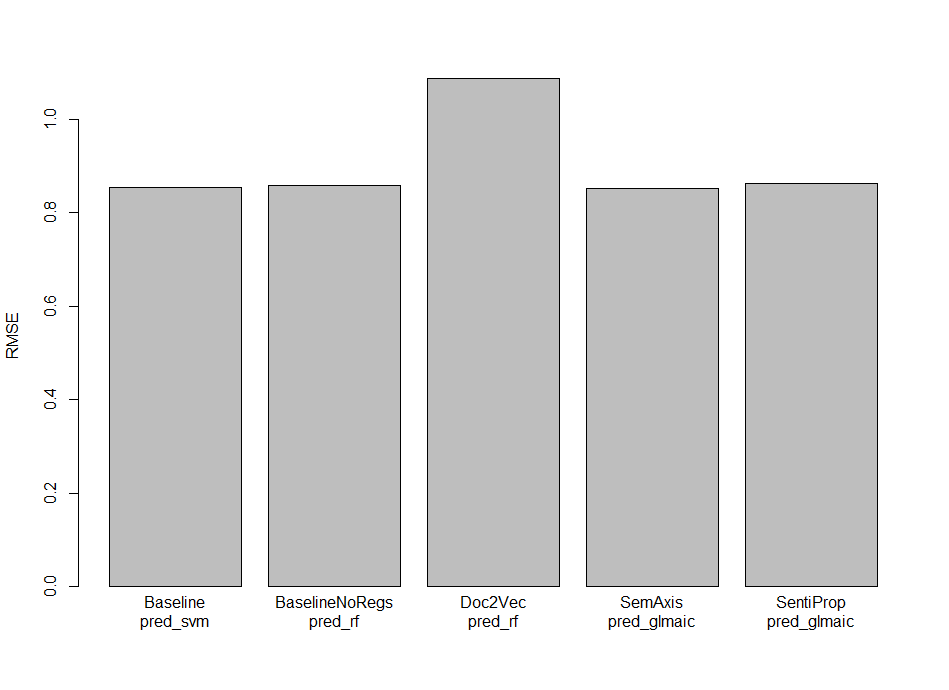
\includegraphics[width=.8\linewidth]{graphs/RMSE.png}
    %     \caption{The RMSE Score of Regression models}
    %     \label{Fig:RMSE}
    % \end{subfigure}
    % \begin{subfigure}{.5\textwidth}
    %     \centering
    %     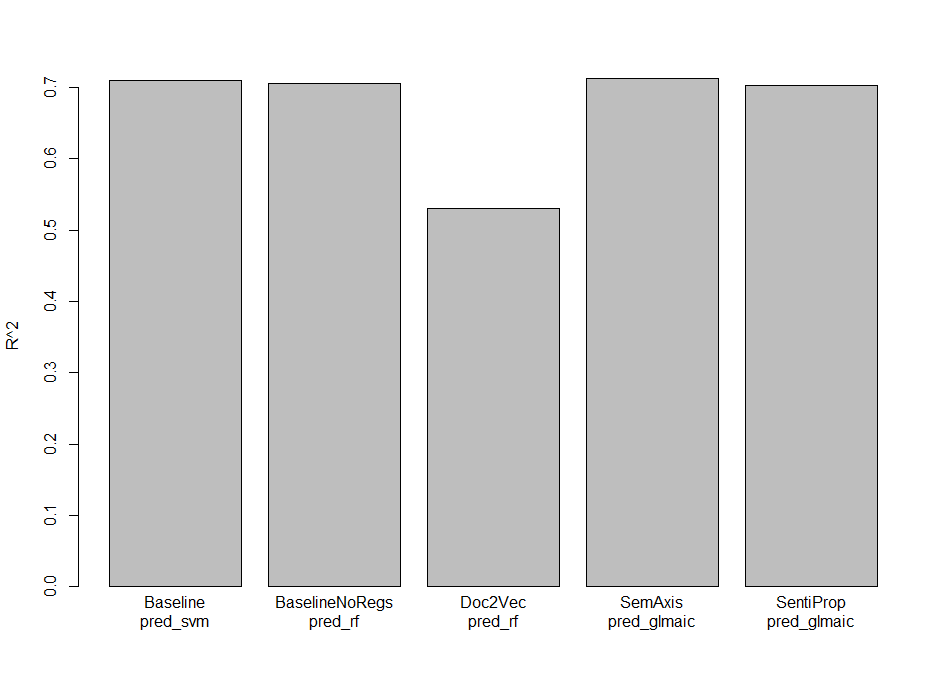
\includegraphics[width=.8\linewidth]{graphs/Rsquared.png}
    %     \caption{The $R^2$ Score of Regression models}
    %     \label{Fig:RSquared}
    % \end{subfigure}
    % \end{figure}
    
    We also calculated the prediction metrics using the holdout set composed of the last three months of the sample. For this holdout set, both the random forest and the MARS model with no regressors achieve the best performances in terms of RMSE ($1.06$-$1.09$) and $R^2$ ($0.41$-$0.4$) as shown in Table \ref{Tab:Volatility2}.
    
    The deterioration in prediction quality by changing the hold out set is evident. The RMSE increases in almost one fourth of the original values and the MAE also shows a slight increase.  The results appear to point once again to the instability of the association between the predictors and the targets. 
    
    \begin{table}[H]
    \centering
    \begin{threeparttable}
   \begin{tabular}{rrrrrrrrr}
      \hline
     & & \textbf{RMSE} & \textbf{R}$^2$ & \textbf{MAE} & & \textbf{RMSE} & \textbf{R}$^2$ & \textbf{MAE}\\ 
      \midrule
      \multirow{8}{*}{\textbf{Baseline}} & & \multicolumn{3}{c}{\textbf{No Regs}} & & \multicolumn{3}{c}{\textbf{McDonald}} \\
      \cmidrule{3-9}\\
      & \textit{GLM} + \textit{AIC} &  1.13 & 0.35 & 0.72 & & 1.16 & 0.34 & 0.76 \\ 
      & \textit{MARS} &  1.09 & 0.40 & \textbf{0.69} & & 1.12 & 0.37 & 0.74 \\ 
      & \textit{RF} & \textbf{1.06} & \textbf{0.41} & 0.76 & & 1.12 & 0.38 & 0.80\\ 
      & \textit{SVM} & 1.11 & 0.39 & 0.70 & & 1.10 & 0.37 & 0.76 \\ 
      \multicolumn{9}{c}{} \\
      \multirow{8}{*}{\textbf{ID}} & & \multicolumn{3}{c}{\textbf{SemAxis}} & & \multicolumn{3}{c}{\textbf{SentiProp}} \\
      \cmidrule{3-9}\\
       & \textit{GLM} + \textit{AIC} & 1.17 & 0.32 & 0.82 &  & 1.14 & 0.35 & 0.78 \\ 
      & \textit{MARS} & 1.19 & 0.33 & 0.83 &  &1.17 & 0.38 & 0.82 \\ 
      & \textit{RF} &  1.11 & 0.36 & 0.80 & & 1.08 & 0.39 & 0.76 \\ 
      & \textit{SVM} & 1.10 & 0.40 & 0.78 & & 1.14 & 0.34 & 0.80 \\
      \multicolumn{9}{c}{} \\
      \multirow{8}{*}{\textbf{Doc2Vec}} & & \multicolumn{3}{c}{\textbf{Doc2Vec}} & & \multicolumn{3}{c}{\textbf{}} \\
       \cmidrule{3-9}\\
      & \textit{GLM} + \textit{AIC} &  1.50 & 0.03 & 1.22 & \multicolumn{4}{c}{} \\ 
      & \textit{MARS} & 1.84 & 0.25 & 1.61 & \multicolumn{4}{c}{} \\
      & \textit{RF} & 1.39 & 0.01 & 1.09 &  \multicolumn{4}{c}{}\\ 
      & \textit{SVM} & 1.44 & 0.02 & 1.18 & \multicolumn{4}{c}{}\\
       \bottomrule
    \end{tabular}
    \begin{tablenotes}
      \footnotesize
      \item GLM + AIC method is based on a stepwise selection procedure applied to a GLM model. MARS is used to denote the multivariate adaptive regression splines algorithm with generalized cross-validation selection. RF stands for the random forest model and SVM for support vector model. ID stands for induced dictionary methods.
    \end{tablenotes}
    \caption{Volatility prediction last three months holdout}
    \label{Tab:Volatility2}
  \end{threeparttable}
    \end{table}
    
    \section{News Freshness}
    
    We created a news freshness index following the explanations given in the methodology, section \ref{NF}. The index is calculated based on the cosine similarity between document embeddings in a given day and an exponentially weighted moving average. 
    
    The plot below shows the evolution of the proposed indexes in the period 2019-2020 against the realized volatility obtained with the $S\&P$ $100$ index. All series are scaled and smoothed using a medium-sized Henderson filter built through the RHKS methodology proposed in \textcite{Dagum:2016}. 
    
    \begin{figure}[H]
    \centering
    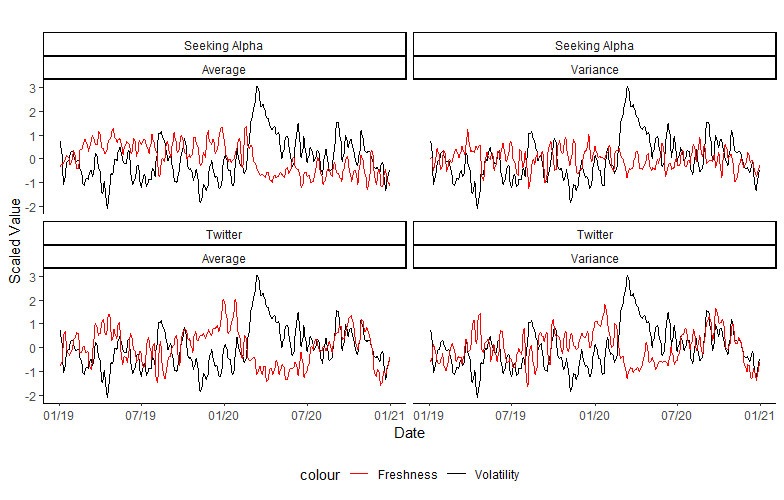
\includegraphics[width=15cm]{graphs/500LineFresh.png}
    \caption{News Freshness Index and realized volatility}
    \label{Fig:LineFresh}
    \end{figure}
    
    As can be seen in Figure \ref{Fig:LineFresh}, indexes of news freshness for both Twitter and Seeking Alpha are highly volatile. Even with a moderate amount of smoothing, all series still present several up's and down's over the considered period. We note that both indexes hit a very low point during march-april of 2020 period, in which the volatility also increased notoriously. The pattern is more evident for indexes based on the daily average of the similarity (left hand side) but also slightly true for the ones based on the average deviation. This latter observation is particularly true for the one derived from Twitter.
    
    Another interesting observation can be made by zooming in the last two months of $2019$. We note that during these period the news freshness index increased notoriously while the realized volatility reduced sharply. 
    
    \begin{figure}[H]
    \centering
    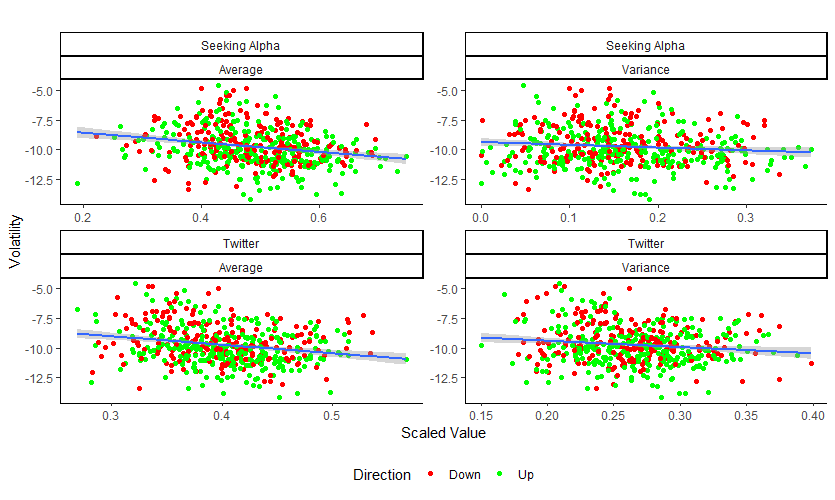
\includegraphics[width=16cm]{graphs/500ScatterFresh.png}
    \caption{News Freshness Index scatterplot}
    \label{Fig:ScatterFresh}
    \end{figure}
    
    Figure \ref{Fig:ScatterFresh} above shows the relation between the realized volatility and the freshness indexes colored by direction. There is a statistically significant negative association between both. We note also, that the relation is quantitatively bigger when using the indexes based on averages rather than variances. There is evidence that volatility reduces when the informational content between news increases. 
    
    Figure \ref{Fig:DistrFresh} shows violin plot for the distributions of the freshness indexes across up and down days. Although some slight differences in the shapes can be seen, there isn't any clear distinction on the span, nor an evident separation between both classes.
    
    \begin{figure}[H]
    \centering
    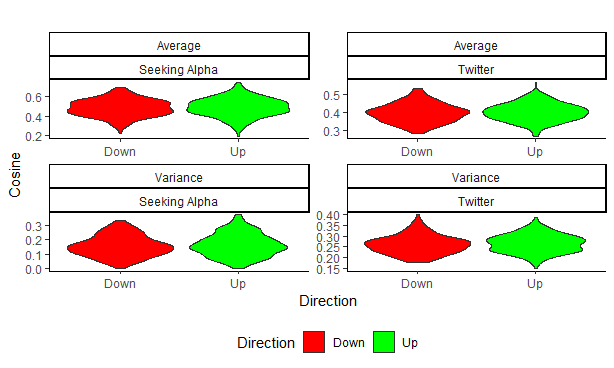
\includegraphics[width=15cm]{graphs/500DistrFresh.png}
    \caption{News Freshness Index distribution across direction}
    \label{Fig:DistrFresh}
    \end{figure}
    
    Table \ref{Tab:Freshness} shows the results of a GLM model estimated using stepwise AIC selection, considering the news freshness indexes and lags.  The baseline model includes only lags of the dependent variable.
    
    The baseline model for the classification task is better than the one obtained using the freshness indexes. The regression model for the volatility shows slightly better results when using the indexes compared with the baseline. We note a slight improvement in the RMSE metric evaluated over the test set. 
    
    Even though the gain of using the freshness indexes is quantitatively small, the lags of both are statistically significant at the $10\%$ level for the volatility regression, as can be seen in table \ref{Tab:FreshnessVol}. A similar result is obtained when solving the classification task as shown in table \ref{Tab:FreshnessDir}. Lags for both average indexes and variance are significant at the $10\%$ level. 
    
    \begin{table}[ht]
    \centering
    \begin{threeparttable}
    \begin{tabular}{rlrrrrrr} 
    &
    \multicolumn{2}{c}{\textbf{Volatility}} & & \multicolumn{4}{c}{\textbf{Direction}}\\
      \toprule
     Metric & RMSE & MAE &  &Accuracy & Precision & Recall & F1  \\ 
      \midrule
    Baseline & 0.89 & \textbf{0.78}& & \textbf{0.66} & 0.66 & \textbf{1.00} & \textbf{0.80}\\ 
    GLM + AIC & \textbf{0.88} & \textbf{0.78} & & 0.61 & \textbf{0.68} & 0.81 & 0.73\\ 
       \bottomrule
    \end{tabular}
    \begin{tablenotes}
      \footnotesize
      \item GLM + AIC method is based on a stepwise selection procedure applied to a GLM model. In the case of the volatility the GLM model is a standard linear regression while for the direction it is a logistic regression. 
    \end{tablenotes}
    \caption{News freshness prediction}
    \label{Tab:Freshness}
  \end{threeparttable}
    \end{table}
    
\begin{table}
\centering
  \begin{threeparttable}
     \begin{tabular}{rrrrl}
      %\toprule
     & \textbf{Estimate} & \textbf{Std. Error} & \textbf{t-val} & \textbf{P-val} \\ 
      \midrule
      \textit{Vol$_{t-1}$} & 0.67 & 0.05 & 13.36 & 0.0000$^{***}$ \\ 
      \textit{Vol$_{t-2}$} & 0.15 & 0.05 & 2.99 & 0.0030$^{***}$ \\ 
      \textit{NFSA$_{t-1}$} & -0.85 & 0.51 & -1.67 & 0.0950$^{*}$ \\
    \textit{NFTW$_{t-1}$}  & -2.05 & 0.96 & -2.14 & 0.0331$^{**}$ \\ 
       \bottomrule
    \end{tabular}
    \begin{tablenotes}
      \footnotesize
      \item Intercept omitted. $NFSA$ stands for the news freshness index obtained with Seeking Alpha aggregating by average. $NFTW$ is the analogous index based on the Twitter corpus.
    \end{tablenotes}
    \caption{Volatility regression}
    \label{Tab:FreshnessVol}
  \end{threeparttable}
\end{table}

\begin{table}
\centering
  \begin{threeparttable}
     \begin{tabular}{rrrrl}
      %\toprule
     & \textbf{Estimate} & \textbf{Std. Error} & \textbf{t-val} & \textbf{P-val} \\ 
      \midrule
      \textit{Dir$_{t-1}$} & -0.47 & 0.21 & -2.22 & 0.0263$^{**}$ \\
      \textit{VNFSA$_{t-2}$} & 2.54 & 1.37 & 1.85 & 0.0644$^{*}$ \\ 
      \textit{NFSA$_{t-3}$} & -1.98 & 1.17 & -1.69 & 0.0904$^{*}$ \\ 
      \textit{VNFTW$_{t-3}$} & -4.86 & 2.56 & -1.90 & 0.0569$^{*}$ \\ 
      \textit{NFTW$_{t-1}$} & 4.86 & 2.21 & 2.20 & 0.0281$^{**}$ \\  
       \bottomrule
    \end{tabular}
    \begin{tablenotes}
      \footnotesize
      \item Intercept omitted. $NFSA$ stands for the news freshness index obtained with Seeking Alpha aggregating by average. $NFTW$ is the analogous index based on the Twitter corpus. Regressors that start with $V$ refer to the news freshness index obtained using the mean average deviation as aggregation.
    \end{tablenotes}
    \caption{Direction classification}
    \label{Tab:FreshnessDir}
  \end{threeparttable}
\end{table}

\section{Trade Strategy}

In this section we show the results obtained by implementing two trade strategies based on the predictions obtained on the random held-out observations. The fist strategy, $\pi$, consists in broad terms of selling the index if the following day the market is predicted to go up, and buying if the market is predicted to go down (we assume short-selling is allowed). Strategy $\pi_\sigma$ implements a volatility correction that lowers the probability of executing the trade in days with high volatility. The way this is implemented is explained in more detail in section \ref{TS}. 

Table \ref{Tab:Trade} shows the gains obtained by using both strategies explained. The index initial value is assumed to be $1$ and the value for each day is derived by applying the compound return rate. 

 \begin{table}[H]
    \setlength{\columnwidth}{1pt}
    \centering
    \begin{threeparttable}
   \begin{tabular}{rrrrrrrrr}
      \hline
     & & $\mathbf{\pi}$ & $\mathbf{\pi_\sigma}$ & $\mathbf{\delta}$ & & $\mathbf{\pi}$ & $\mathbf{\pi_\sigma}$ & $\mathbf{\delta}$ \\ 
      \midrule
      & & \multicolumn{3}{c}{\textbf{AdaBoost}} & & \multicolumn{3}{c}{\textbf{SVM}} \\
      \cmidrule{3-9}\\
      & \textit{McDonald} & -0.01 & 0.14 & 0.15 & & -0.03 & 0.04 & 0.07 \\ 
      & \textit{No Regs} & -0.03 & 0.13 & 0.15 & & 0.26 & 0.22 & -0.04  \\ 
      & \textit{Doc2Vec} & 0.24 & 0.10 & -0.14 & & 0.26 & 0.20 & -0.06 \\ 
      & \textit{SemAxis} & 0.26 & 0.22 & -0.04 & & 0.36 & \textbf{0.46} & 0.09  \\ 
      & \textit{SentiProp} & \textbf{0.45} & 0.34 & -0.11 & & 0.26 & 0.27 & 0.02 \\ 
      \multicolumn{8}{c}{} \\
      & & \multicolumn{3}{c}{\textbf{RF}} & & \multicolumn{3}{c}{\textbf{GLM + AIC}} \\
      \cmidrule{3-9}\\
       & \textit{McDonald} & -0.03 & 0.10 & 0.14 & & 0.07 & 0.21 & 0.14 \\ 
      & \textit{No Regs} & 0.02 & 0.13 & 0.11 & & 0.09 & 0.11 & 0.02  \\ 
      & \textit{Doc2Vec} & 0.26 & 0.33 & 0.07 & & 0.03 & 0.07 & 0.03 \\ 
      & \textit{SemAxis} & 0.35 & 0.16 & -0.19 & & -0.13 & -0.01 & 0.12\\ 
      & \textit{SentiProp} & 0.18 & 0.31 & 0.13 & & 0.13 & 0.16 & 0.03  \\ 
       \bottomrule
    \end{tabular}
    \begin{tablenotes}
      \footnotesize
      \item Shows the gains of the trade strategies proposed in section \ref{TS} with a initial index value of $1\$$. The $\delta$ column shows the difference between the gains of strategy $\pi_\sigma$ against $\pi$.  
    \end{tablenotes}
    \caption{Trade strategy gains}
    \label{Tab:Trade}
  \end{threeparttable}
    \end{table}
    
    Results obtained show that the SentiProp method with the AdaBoost model achieves the best results in terms of gains, $0.45$ cents over the two years included in the sample. The second best is the combination of the SemAxis method with the SVM model. As can be seen the best combinations of methods and models in terms of statistical metrics differ with those that achieve the best performance on the trade strategy. The difference arises because dissimilarities in the magnitude of the returns.  

    Gains are on average higher across all methods and models when using the volatility corrected trade strategy. The only notable exceptions are the SemAxis method with the RF model and the Doc2Vec method with the AdaBoost model. The use of the volatility corrected strategy improves the gains both the McDonald and the No Regs methods across all models considered. The new best combination with this strategy is the SemAxis $+$ SVM with a gain of $0.46$. 
    
    \begin{figure}[H]
    \centering
    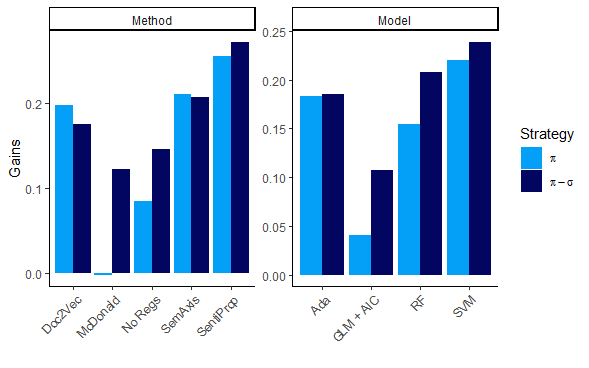
\includegraphics[width=15cm]{graphs/TradeAgg.png}
    \caption{Trade strategy aggregated gains}
    \label{Fig:TradeAgg}
    \end{figure}
    
    Figure \ref{Fig:TradeAgg} shows the average of the gains obtained, aggregating by both method and model for each of the strategies. We note that aggregating by method, the gains are slightly reduced for the Doc2Vec method and the SemAxis when using the volatility corrected strategy $\pi_\sigma$. However, the gains increase significantly for the other methods. On average the best method across models is the SentiProp, result which coincides with the one obtained through the statistical metrics. 
    
    When summarising across models, we note that the average gain is increased by using the volatility corrected strategy. The additional gain for changing the strategy is bigger for the GLM $+$ AIC model. Overall, the SVM model is the one that has a higher gain with both strategies. This result is also the same as the one we obtained when evaluating the predictions only in terms of statistical metrics (see section \ref{Sec:Dir}).
    
    \begin{figure}[H]
    \centering
    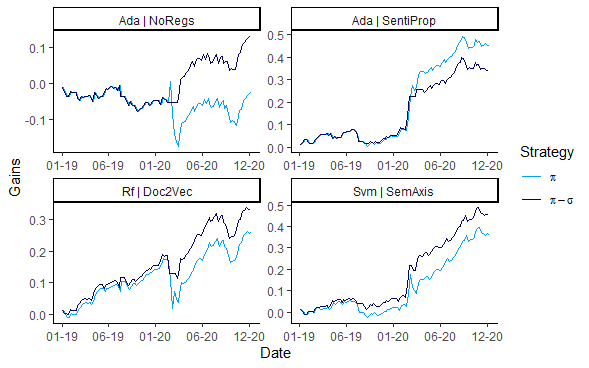
\includegraphics[width=15cm]{graphs/Strategies.png}
    \caption{Trade strategies cumulative gains}
    \label{Fig:TradeLine}
    \end{figure}

    Figure \ref{Fig:TradeLine} shows the cumulative returns obtained with both strategies for a set of methods and models in which the change of strategy reflects in the biggest difference in gains. In the top right panel for the AdaBoost model with SentiProp method, the volatility corrected strategy achieves a lower total gain as some of the trades that were supposed to be carried out during march of 2020 and ended up in gains were not done. In the other three panels some trades that ended up in losses during the start of the covid-19 pandemic were not done due to the high volatility and hence the overall gains are higher with the corrected strategy, $\pi_\sigma$, that with the non-corrected one.
    
    Overall, results suggest that during the first sixth months of $2020$ there were several trade opportunities that could have generated gains. 
    
    
    
    \chapter{Conclusion}
    
    As some reviews have already established, (see for instance, \textcite{Nassirtoussi:2014}) the relation between textual sentiment and market returns depends on the source of the textual information used and the sample considered. We tried to limit ourselves to sources that were easily available and to the most recent sample. We found that when using a regular hold-out set prediction accuracy obtained is very close to the no-information rate. A slight improvement in prediction performance is obtained when using the last three months in the sample as holdout set. All in all, our results show that for the source and sample considered, prediction gains obtained by the use of textual information are small. This is in contrast to results that have been usually found in the field, see \textcite{Kearney:2014}. It might be worth investigating further if the relation between text sentiment and how investor behavior has been modified due to the covid-19 pandemic. 
    
    After the article of \textcite{Antweiler:2004}, we are one of the few that tries to establish a relation between textual sentiment and volatility. We find that sentiment series derived from both traditional methods and induced dictionaries slightly improve forecast accuracy. Our focus is more on predictive efficiency rather than statistical inference (as others in the field). Results obtained for the realized volatility are still highly dependent on the hold-out set used. In contrast to the results obtained for the classification task, models trained excluding the three last months of the sample have a lower prediction accuracy for the volatility. 
    
    We propose an index of informational content that has a negative association with realized volatility. However, informational content doesn't appear to be related with market direction. Forecast improvement obtained by using the proposed freshness index is very modest, though statistical inference suggests that the association between both is statistically significant. Up to our knowledge we are the first that propose using a freshness index to measure current informational content in the market. We are convinced that there are a lot of research opportunities in this area and that there is a strong financial intuition to argue the negative relation between volatility and this type of indexes.  
    
    Trade strategies based on textual sentiment have been regularly used in the field to evaluate results obtained. \textcite{Engelberg:2012} proposed a trade strategy that generated a return of approximately $180\%$ on the 2 year sample analyzed. We obtain more modest returns (approximately $45\%$ in the best case scenario) with our proposed strategy, but still show that its possible to obtain above-average gains based on the predictions derived from textual sentiment. It is important to take into account that a great part of the gains were obtained during the first four months of the pandemic which strongly suggests that there might be opportunities to obtain abnormal returns during market crisis times. A result that was shown before by \textcite{Garcia:2013}. Furthermore, we find evidence that gains can be improved on average by incorporating information of the current volatility in the market. 
    
    Our document incorporates several advancements in methodological terms, compared to techniques used in the field. One of the strongest suggestions of the review made by \textcite{Kearney:2014} is that it was crucial to generate word lists that were more authoritative than the \textcite{Loughran:2011}, to capture negative sentiment in the future and that it was necessary to start using better weighting schemes for these. We addressed both problems by applying methodologies of dictionary induction for each of the text sources considered. We also propose, up to our knowledge, one of the first uses of word embeddings in order to derive textual sentiment in the financial field. 
    
    A possible future line of research is the time varying relation between textual sentiment and investor behavior. In particular, it would be interesting to study whether this relationship was  modified due to the covid-19 pandemic. Another interesting research question that remains open is whether there exists reverse causation between stock prices and news articles (as was studied in \textcite{Garcia:2013}) and if this relation has a different magnitude during financial crisis. 

    % FUTURE RESEARCH
    % It would be interesting to study reverse causation between stock prices and news based on Garcia 2012
    % We made important advances in term of methodology. Use of embeddings.  Kearney suggest that is important to generate more authoritative word lists than the L&M and to use better weighting schemes. We address both problems by inducing a new set of dictionaries based on the used sources. 
    % A possible future line of research is the time varying relation between textual sentiment and investor behavior (covid might have induced a change in the relation)
    
    
    % Ideas
    
    %DIRECTION
    % We believe that results obtained in regard to the relation of market variables and news are heavily dependent on both the sample considered and the source of the textual information. Most papers in the field don't use freely available sources we are one of the few that use these and find a slightly improvement of performance compared with the no information rate when using the last 3-months holdout.
    %  
    
    % VOLATILITY
    % After \textcite{Antweiller} we are one of the few papers that tries to establish a relation between textual sentiment and volatility. We find that sentiment series derived from both traditional methods and induced dictionaries slightly improve forecast accuracy. We focus more on predictive abilities rather than inference (change of perspective). 
    % Results obtained are highly dependent on the hold-out set used. We find that models trained excluding the three last months of the sample have a lower prediction capacity. 
    
    %INFORMATIONAL CONTENT
    % We propose an index of informational content that has a negative association with realized volatility. However, the informational content doesn't appear to be related with the market direction. Forecast improvement by using the freshness index is very modest though statistical inference suggests that the association is statistically significant. 
    % We are one of the first to propose generating an informational content index. We believe that there are a lot of research opportunities related to this topic and it makes sense to think that more informational content should reduce market volatility.
    
    %TRADE STRATEGIES
    % Trade strategies based on textual sentiment have been regularly used in the field to evaluate results obtained. Engelberg et al 2012 proposed a trade strategy that generated a return of $180%$ on a 2 year sample. We obtain more modest returns but still show that its possible to obtain gains based on the predictions derived from the textual sentiment. 
    % A great part of the gains are obtained during the first four months of the pandemic which suggests that there might be opportunities to obtain abnormal returns during market crisis times as Garcia 2012
    % We find evidence that taking into account information of the volatility trade gains can be augmented. 
    
    %FUTURE RESEARCH
    % It would be interesting to study reverse causation between stock prices and news based on Garcia 2012
    % We made important advances in term of methodology. Use of embeddings.  Kearney suggest that is important to generate more authoritative word lists than the L&M and to use better weighting schemes. We address both problems by inducing a new set of dictionaries based on the used sources. 
    % A possible future line of research is the time varying relation between textual sentiment and investor behavior (covid might have induced a change in the relation)
    
    
    
    %\begin{comment}
    %\section{Important Ideas}
    
    %\subsection{Data}
    
    %We have 
    %\begin{itemize}
    %    \item {Seeking Alpha US Markets: 4700 news for the two %years.}
    %    \item {WSJ: 35000 news for the two years. }
    %    \item {Twitter: 42000 tweets}
    %\end{itemize}
    
    %\textbf{It would be interesting if exploration could be done using not only LDA but also LSA}
    
    %\textbf{Good ideas on further questions to explore could be found in \textcite{Ke:2019}}
    
    
    %\subsection{Methodology Features}
    %Dictionary methods can be understood as an unsupervised feature selection that acts at the bag of words level. We could do better if we could let the model decide what to use but then the BOW representation is high-dimensional and too sparse for things to work out. A preliminary approach could be using a Naive Bayes as in \textcite{Antweiler:2004}.
    
    %A simple solution is given in \textcite{Ke:2019} with what they call "Predictive Screening" we could use this method to create a Good|Bad word seed set. \textbf{A decision would have to be taken regarding the choice of hyperparameters, i.e thresholds for what we call "useful" and minimum number of appearances of the word so as not to capture very infrequent words}. In that paper they use a two topic generative model à la LDA. The model could be made with our data \textbf{if we could match seeking alpha news to each company}.
    
    %\textbf{The creation of the seed set based on predictive screening could allow us to use the two semi-supervised induction methods} that we have ready \textcite{Hamilton:2016} and \textcite{An:2018}. In the \textcite{Xing:2018} review there is a mention to another paper in the field Tai-Kao I haven't read it and don't know if we should explore that one.
    
    %Probably the most accurate option could be letting go of the idea of sentiment analysis and start working directly at the feature level. Again BOW has the same problems as above plus that it breaks the context|relation between words. \textbf{We could use word embeddings to preserve semantic relations possibly GloVe \textcite{Pennington:2014}  and word2vec \textcite{Mikolov:2013}}. \textbf{Once we have the word embeddings we could use a classifier but again the high dimensionality problem would persist}. To address this we could the doc2vec method \textcite{Le:2014} or we could try using the sentence embedding in \textcite{Arora:2019} or a simple average over the semantic space. One very interesting option would be \textcite{Gupta:2020} it seems perfectly tailored for our problem but I am starting to think that it might overfit so we would have to be careful with the train-test split.
    
    %\section{Methodology Estimation}
    %No need to go that far the literature suggest that naive bayes + support vector machines should be enough. For the variance problem we could definitely try using support vector regression. Probably we could work on pre-whitened residuals at the series level. \textcite{Nassirtoussi:2014}
    
    %A simple way to make some sort of initial exploration is using the github code in \textcite{Sun:2016}.
    
    %We just have the 600 points for the daily financial series and there is an evident regime change in 2020 so I think we should just dismiss any neural network approach. 
    
    %\textcolor{blue}{Blue comments are made by Daniel}
    %\end{comment}
    
\printbibliography
\clearpage

\appendix
\chapter{Appendix}
%\Huge{Appendix}
\normalsize
%Code Appendix

\begin{longtable}{p{1.5cm}p{7cm}p{3cm}p{1.5cm}}
\caption{LDA Results of WSJ}
\hline
Topic Number & Keywords & Topic Name & Selection \\
\hline
0 & \multicolumn{1}{m{6cm}}{china, trade, country, government, tariff, trump, president, chinese, official, economic} & Trade War & Y \\
\hline
1 & \multicolumn{1}{m{6cm}}{state, department, federal, official, program, mayor, cuomo, increase, city, california} & US Politics & N \\
\hline
2 & \multicolumn{1}{m{6cm}}{company, billion, business, financial, investment, million, credit, investor, money, accord} & Investment, Company & Y \\
\hline
3 & \multicolumn{1}{m{6cm}}{company, facebook, google, user, information, platform, people, include, group, product} & Technology Company & Y \\
\hline
4 & \multicolumn{1}{m{6cm}}{trump, president, house, white, administration, official, justice, court, department, committee} & Trump, Election & N \\
\hline
5 & \multicolumn{1}{m{6cm}}{mexico, border, farmer, migrant, immigration, asylum, mexican, immigrant, bayer, country} & Military, National Security & N \\ 
\hline
6 & \multicolumn{1}{m{6cm}}{house, family, brexit, johnson, artist, years, couple, design, museum, credit} & Life & N \\ 
\hline
7 & \multicolumn{1}{m{6cm}}{player, sport, league, season, european, italy, europe, game, world, country} & Sports & N \\ 
\hline
8 & \multicolumn{1}{m{6cm}}{economy, market, rates, economic, investor, yield, month, banks, growth, bond} & Economics & Y \\ 
\hline
9 & \multicolumn{1}{m{6cm}}{company, worker, sales, employee, executive, chief, business, million, pandemic, billion} & Retail & Y \\   
\hline
10 & \multicolumn{1}{m{6cm}}{police, officer, people, protest, kill, press, protester, official, associate, arrest} & Police & N \\    
\hline
11 & \multicolumn{1}{m{6cm}}{court, charge, prosecutor, attorney, investigation, lawyer, federal, allege, judge, comment} & Court, Law & N \\     
\hline
12 & \multicolumn{1}{m{6cm}}{water, minutes, plastic, bottle, chicken, drink, serve, flavor, produce, sugar} & Life, Recipe & N \\   
\hline
13 & \multicolumn{1}{m{6cm}}{school, student, child, family, parent, college, education, teacher, university, class} & Education, School & N \\ 
\hline
14 & \multicolumn{1}{m{6cm}}{company, billion, million, apple, business, technology, revenue, executive, disney, include} & Business, Companies & Y \\ 
\hline
15 & \multicolumn{1}{m{6cm}}{company, airline, vehicle, boeing, maker, plane, industry, tesla, plant, flight} & Airline & N \\ 
\hline
16 & \multicolumn{1}{m{6cm}}{price, company, market, share, investor, billion, analyst, quarter, stocks, stock} & Companies, Investment & Y \\    
\hline
17 & \multicolumn{1}{m{6cm}}{store, sales, brand, restaurant, product, retailer, customer, company, consumer, online} & Retail & Y \\  
\hline
18 & \multicolumn{1}{m{6cm}}{trump, election, republican, democrat, president, campaign, party, democratic, state, biden} & Election, Politics & N \\     
\hline
19 & \multicolumn{1}{m{6cm}}{china, chinese, huawei, korea, north, government, official, beijing, south, security} & Chinese Technology & Y \\   
\hline
20 & \multicolumn{1}{m{6cm}}{market, trading, investor, stock, trade, exchange, trader, option, stocks, funds} & Market, Trading & Y \\  
\hline
21 & \multicolumn{1}{m{6cm}}{coronavirus, people, case, virus, state, health, covid19, pandemic, hospital, test} & COVID-19 & Y \\  
\hline
22 & \multicolumn{1}{m{6cm}}{university, woman, people, years, black, think, thats, youre, experience, professor} & University, Ethic Equality & N \\      
\hline
23 & \multicolumn{1}{m{6cm}}{official, saudi, military, force, government, state, country, russia, attack, trump} & Military & N \\   
\hline
24 & \multicolumn{1}{m{6cm}}{vaccine, patient, health, study, covid19, people, doctor, medical, disease, treatment} & COVID-19 & Y \\
\hline
25 & \multicolumn{1}{m{6cm}}{million, property, building, accord, hotel, office, market, realestate, owner, space} & Housing, Property & N \\  
\hline
\end{longtable}
\label{tab:LDA}


GitHub repository: \url{https://github.com/lse-st498/Stock-Market-2020-21}

    \begin{sidewaystable}
    \centering
    \caption{Results of SemAxis and SentiProp (WSJ)}
    \scalebox{1}{
    \begin{tabular}{|l|l|l|l|l|l|l|l|} 
    \hline
    Methodology & Embedding & Pos & Neg & PosWords & PosScores & NegWords & NegScores \\ 
    \hline
    \multirow{8}{*}{SemAxis} & \multirow{4}{*}{PT} & F & F & startup, investments, venture… & $\leqslant$ 0.089 & suggested, suggest, worsen… & $\geqslant$ -0.083 \\
    &  & NF & F & startup, venture, venture-backed… & $\leqslant$ 0.089 & suggested, suggest, simulate… & $\geqslant$  -0.085 \\
    &  & F & NF & investments, startup, investing… & $\leqslant$ 0.087 & worsen, suggested, eased… & $\geqslant$ -0.076 \\
    &  & NF & NF & startup, investments, venture... & $\leqslant$ 0.084 & suggested, eased, suggest… & $\geqslant$ -0.078 \\ 
    \cline{2-8}
    & \multirow{4}{*}{ST} & F & F & startup, realty, ventures… & $\leqslant$ 0.157 & relaxing, moderate, eased… & $\geqslant$ -0.154 \\
    &  & NF & F & startup, california-based, scooter… & $\leqslant$ 0.158 & moderate, relaxing, eased… & $\geqslant$ -0.155 \\
    &  & F & NF & developer, startup, holdings… & $\leqslant$ 0.155 & relaxing, eased, dire… & $\geqslant$ -0.152 \\
    &  & NF & NF & developer, startup, california-based… & $\leqslant$ 0.151 & eased, moderate, relaxing… & $\geqslant$ -0.147 \\ 
    \hline
    \multirow{8}{*}{SentiProp} & \multirow{4}{*}{PT} & F & F & risen, project, fund & $\leqslant$ 0.777 & medicine, strategist, severe… & $\geqslant$ 0.168 \\
    &  & NF & F & risen, fund, silicon… & $\leqslant$ 0.742 & affect, strategist, expressed… & $\geqslant$ 0.171 \\
    &  & F & NF & fund, portfolios, investments… & $\leqslant$ 0.742 & restaurant, medicine, strategist… & $\geqslant$ 0.185 \\
    &  & NF & NF & fund, silicon, portfolios & $\leqslant$ 0.723 & restaurant, affect, strategist… & $\geqslant$ 0.190 \\ 
    \cline{2-8}
    & \multirow{4}{*}{ST} & F & F & producer, startup, pipeline… & $\leqslant$ 0.756 & medicine, strategist, severe… & $\geqslant$ 0.157 \\
    &  & NF & F & fund, energy, pipeline… & $\leqslant$ 0.734 & medicine, affect, limit… & $\geqslant$ 0.165 \\
    &  & F & NF & fund, investments, startup… & $\leqslant$ 0.746 & medicine, restaurant, strategist… & $\geqslant$ 0.175 \\
    &  & NF & NF & fund, investments, etf… & $\leqslant$ 0.730 & medicine, restaurant, affect… & $\geqslant$ 0.184 \\
    \hline
    \end{tabular}
    }
    \begin{tablenotes}
    \footnotesize
    \item PT in Embeddings refers to pre-trained embedding, and ST refers to self-trained embedding; F and NF in Pos and Neg mean if the uncertain positive/ negative words are filtered. PosWords and NegWords contain 3 the most positive/ negative words while the PosScores and NegScores refer to the extreme values of corresponding words.
    \end{tablenotes}
    \label{Tab: WSJ senti words}
    \end{sidewaystable}

\newpage





\end{document}
